\chapterimage{10_Dvolom3.jpg} % Chapter heading image

\chapter{Optika v anizotropnih snoveh}
\label{chap:AnizotropneSnovi}
V tem poglavju bomo spoznali optično anizotropne snovi, katerih odziv na 
vpadno svetlobo je odvisen od njene polarizacije. Opisali bomo 
širjenje svetlobe skozi anizotropne snovi in pojasnili razliko med optično 
enoosnimi in optično dvoosnimi snovmi. Spoznali bomo dvojni lom in 
na koncu poglavja predstavili nekaj načinov uporabe tega zanimivega pojava.

\section{Anizotropne snovi}
Do zdaj smo obravnavali izotropne snovi, v katerih je lomni količnik 
snovi enak v vseh smereh in za vse polarizacije vpadne svetlobe. 
Za anizotropne snovi pa je značilno, da imajo 
v različnih smereh različne lastnosti, na primer mehanske, toplotne, 
električne, magnetne, optične ... Primeri optično 
anizotropnih snovi so kremen, kalcit, led, sljuda, tekoči kristali
in tudi raztegnjeni polimerni vzorci, na primer celofan ali prozorni lepilni trak. 
Optično anizotropne snovi najlaže prepoznamo po barvitih vzorcih med
polarizatorjema, ki spreminjajo barvo, ko polarizatorja sučemo. 
Zakaj je tako, bomo spoznali v nadaljevanju poglavja.
\begin{figure}[ht]
\centering
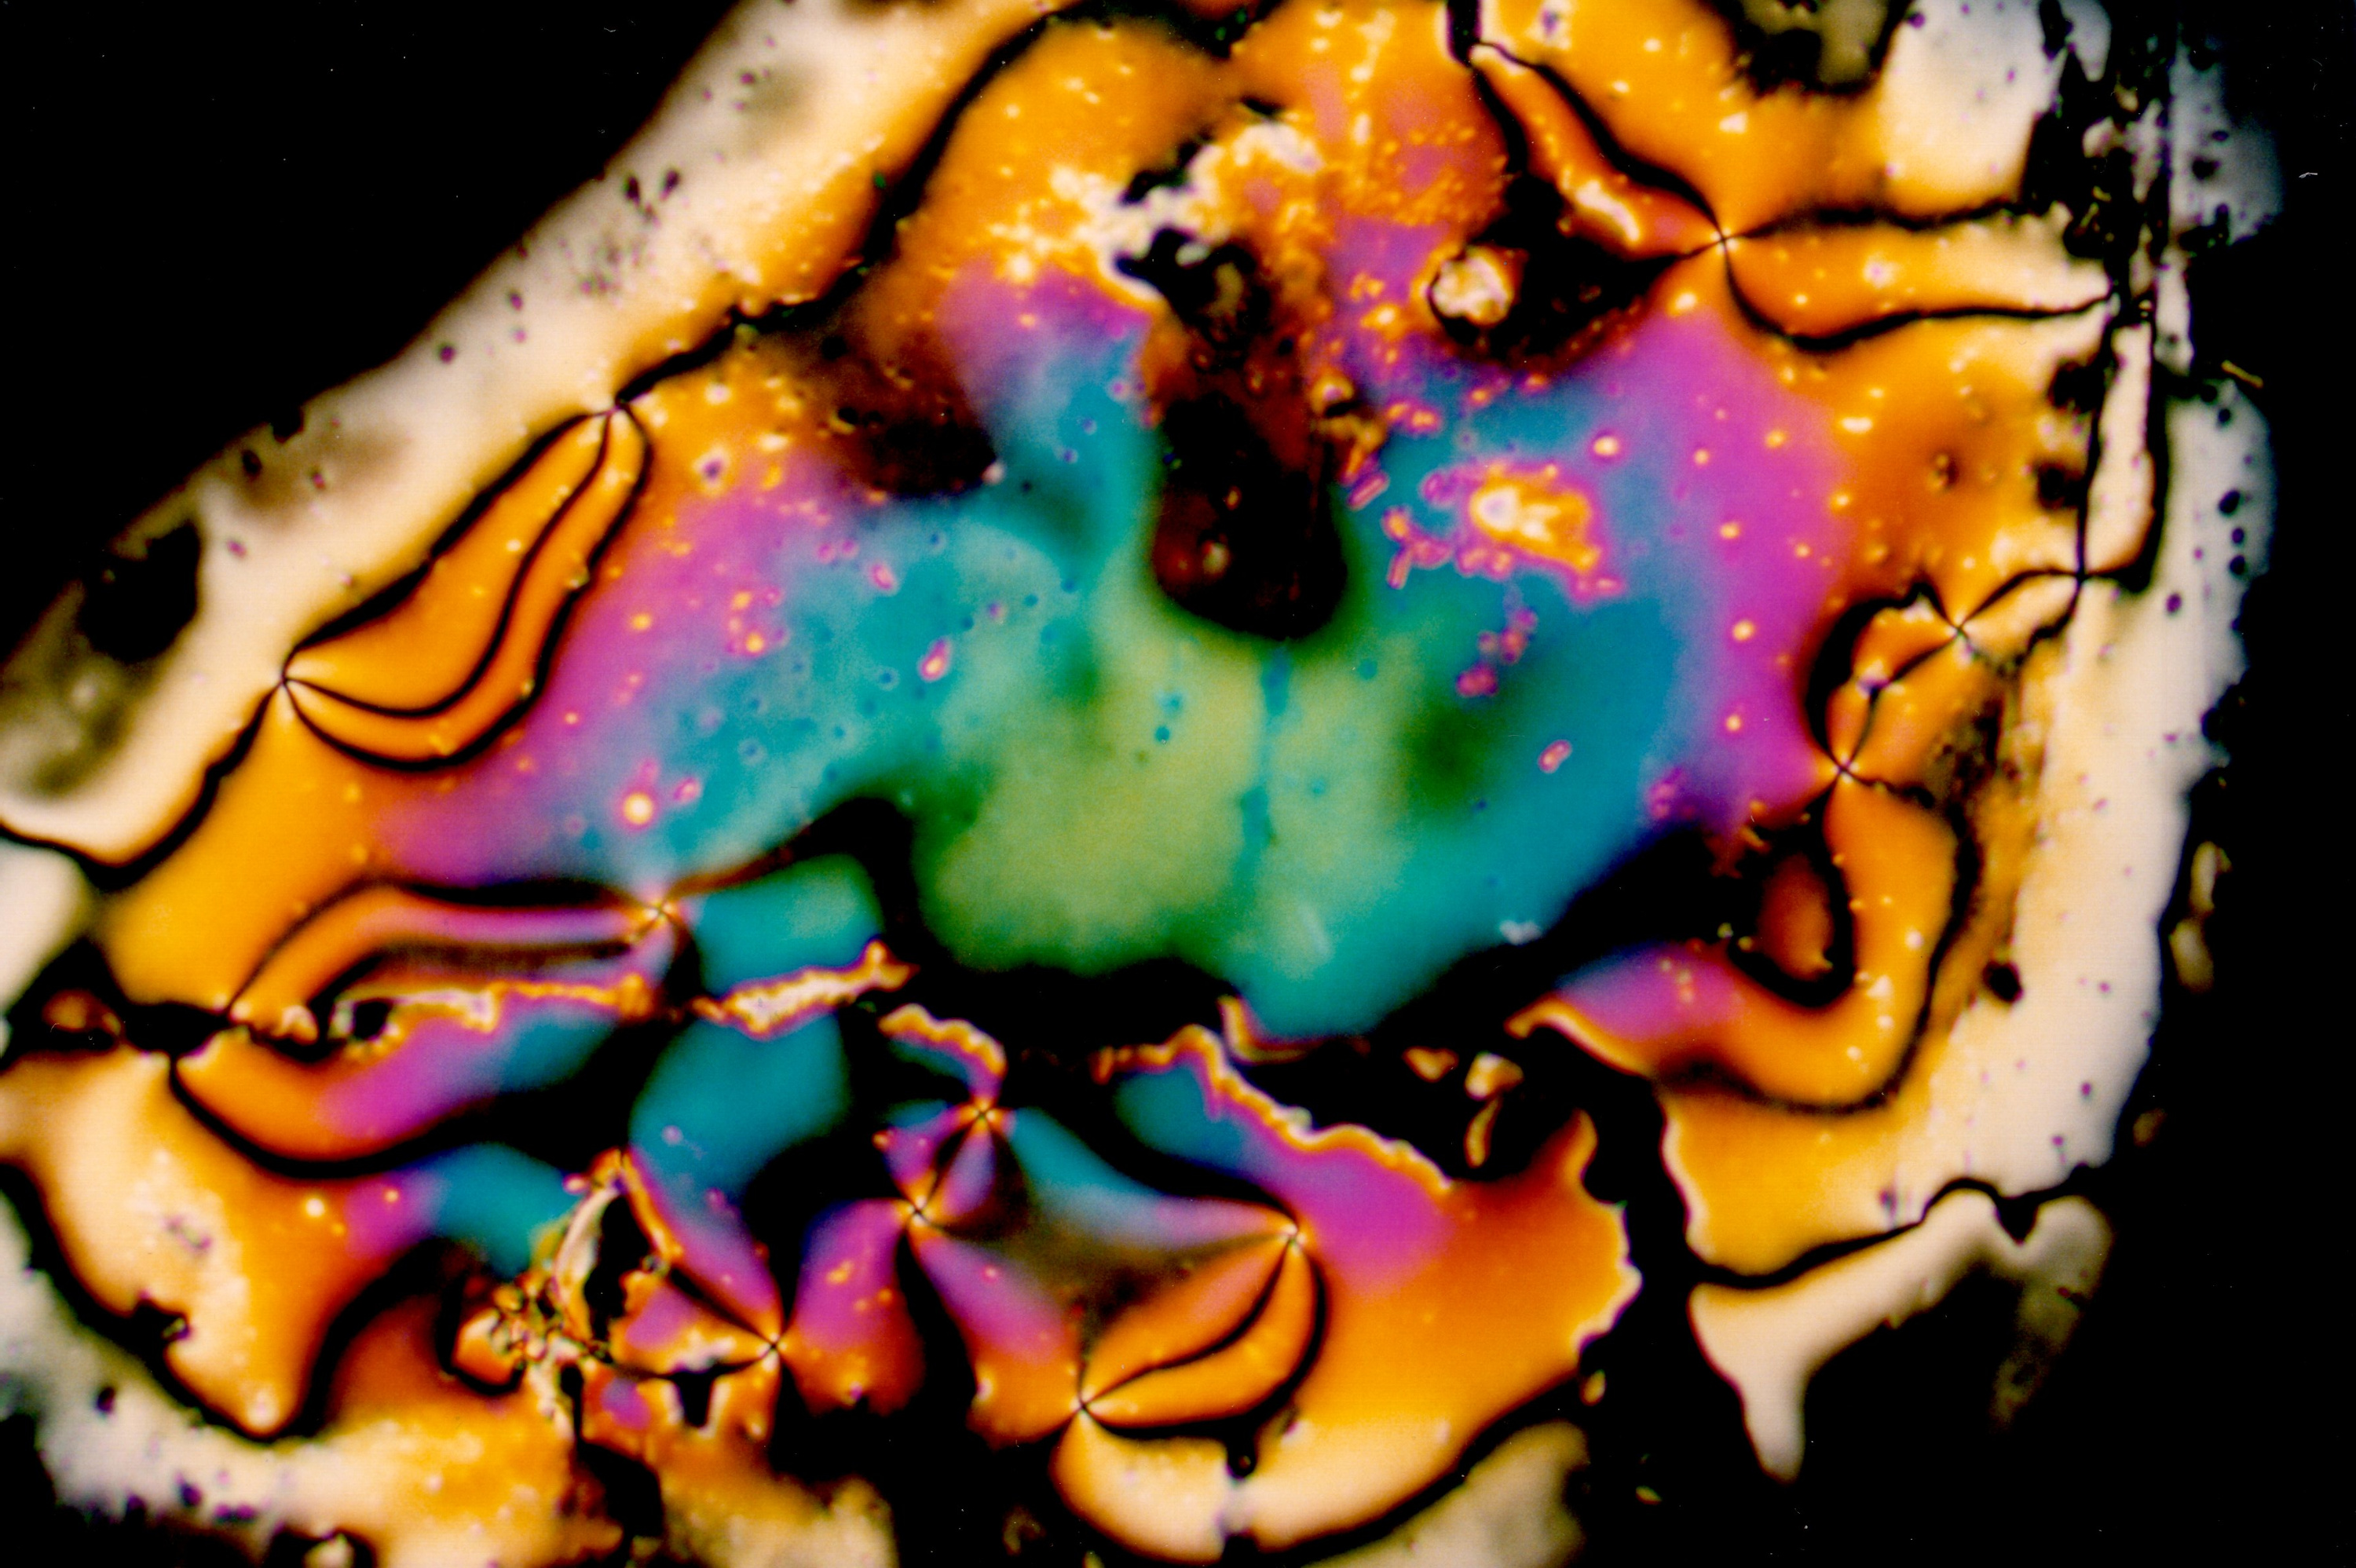
\includegraphics[width=7truecm]{slike/10_foto_nematik.jpg}\hfill
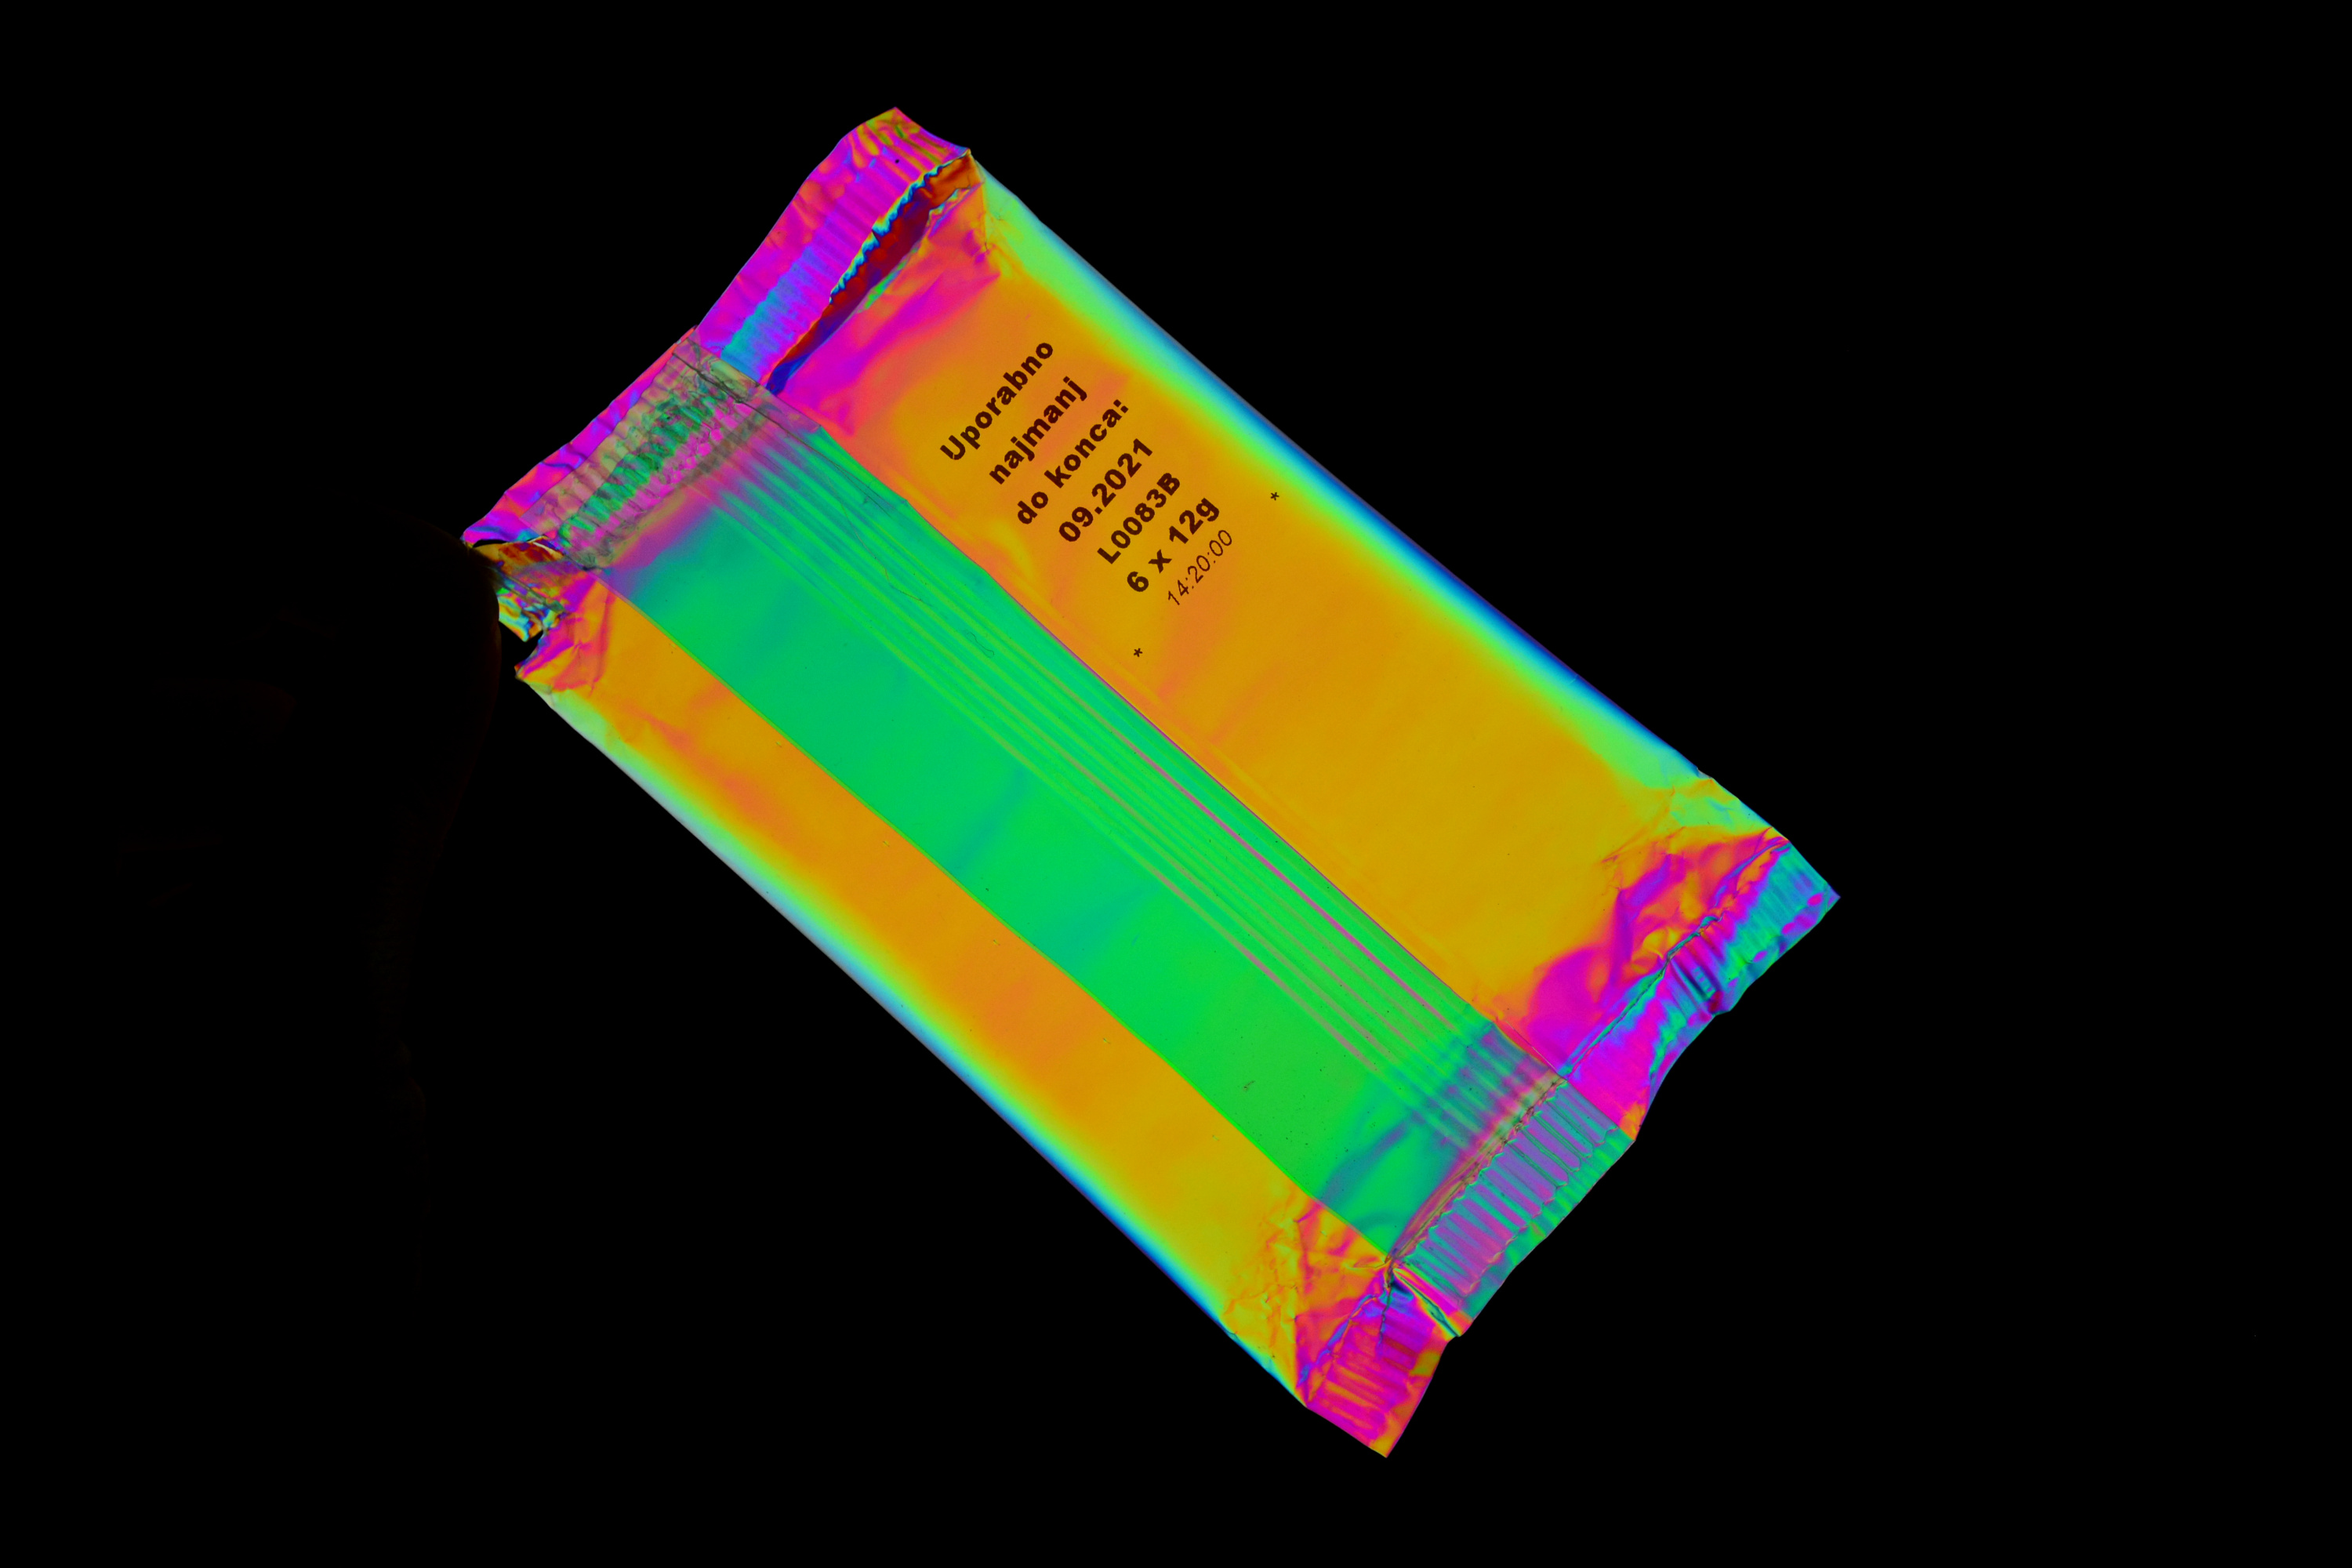
\includegraphics[width=7truecm]{slike/10_foto_celofan.jpg}
\caption{Kapljica tekočega kristala, ki je anizotropna tekočina, slikana pod 
mikroskopom (levo) in ovitek iz celofana (desno). Oba vzorca sta bila postavljena
med prekrižana polarizatorja.}
\label{fig:10_nematik}
\end{figure}

Najznačilnejša optična lastnost anizotropnih snovi je odvisnost lomnega
količnika od smeri širjenja svetlobe in njene polarizacije. Pojav
je posledica odziva snovi na vpadno svetlobo, pri katerem smer in 
velikost inducirane električne polarizacije določa struktura snovi.  
Za nazorno razlago se ponovno poslužimo
Lorentzevega modela, ki smo ga podrobneje spoznali v prejšnjem 
poglavju (glej razdelek~\ref{chap:lomni}). 

Zamislimo si negativno nabito kroglico, ki predstavlja elektron, vpeto v 
mrežo mirujočih sosednjih kroglic, ki predstavljajo pozitivne ione kristala. 
Vzmeti, ki kroglice medsebojno povezujejo, niso vse enake, ampak imajo različne 
konstante vzmeti, odvisno od smeri (slika~\ref{fig:10_model}\,a). Ko na elektron
vpade svetloba, ga sila električnega polja izmakne iz ravnovesne lege, tej sili 
pa nasprotujejo sile vzmeti. Premik elektrona je večji v smeri šibkejše vzmeti, 
zato dipolni moment, ki ga povzroči premik elektrona, ni vzporeden jakosti 
vpadnega električnega
polja. 
\begin{figure}[!h]
\centering
\def\svgwidth{120truemm} 
\input{slike/10_Lorentz_a.pdf_tex}
\caption{Anizotropijo snovi lahko pojasnimo z Lorenzevim modelom, v katerem so
konstante vzmeti, s katerimi je v snov vezan elektron, različne  in $k_1 \neq k_2 \neq k_3$ (a).
V anizotropnih snoveh inducirana električna polarizacija $\mathbf{P}$ ni vzporedna 
z jakostjo električnega polja $\mathbf{E}$ (b).}
\label{fig:10_model}
\end{figure}

Osnovna posledica anizotropnega odziva je, da smer inducirane električne polarizacije $\mathbf{P}$
 v anizotropnih snoveh ni vzporedna smeri jakosti optičnega električnega polja $\mathbf{E}$ 
(slika~\ref{fig:10_model}\,b). Posledično tudi 
vektor gostote električnega polja $\mathbf{D}$ ni vzporeden s smerjo $\mathbf{E}$. 
Linearni odziv snovi zapišemo kot:
\beq
\mathbf{D} = \varepsilon_0 \mathbf{E} + \mathbf{P} = \varepsilon_0 \underline{\varepsilon} \mathbf{E}.
\label{eq:10_001}
\eeq
Vpeljali smo tenzor dielektričnosti $\underline{\varepsilon}$, ki je v anizotropnih snoveh na splošno 
tenzor drugega ranga:
\beq
\underline{\varepsilon} = 
\left[\begin{array}{ccc}
\varepsilon_{xx} & \varepsilon_{xy} & \varepsilon_{xz}\\
\varepsilon_{yx} & \varepsilon_{yy} & \varepsilon_{yz}\\
\varepsilon_{zx} & \varepsilon_{zy} & \varepsilon_{zz}\\
\end{array}\right]\!\!.
\label{eq:10_002}
\eeq
\begin{remark}
Pri obravnavi se bomo omejili na prozorne optično neaktivne anizotropne snovi. 
Ker dielektričnost nastopa v izrazu za energijo elektromagnetnega polja 
(enačba~\ref{eq:03_27}), je zaradi ohranitve energije tenzor $\underline{\varepsilon}$ na splošno
Hermitski in pozitivno definiten. V našem primeru to pomeni, da je 
tenzor simetričen in ga lahko vedno diagonaliziramo, pri čemer so 
vse njegove lastne vrednosti realne in pozitivne.
\end{remark}

Tenzor dielektričnosti diagonaliziramo in v lastnem koordinatnem 
sistemu ga zapišemo kot:
\beq
\underline{\varepsilon} = 
\left[\begin{array}{ccc}
\varepsilon_{xx} & 0 & 0\\
0 & \varepsilon_{yy} &0\\
0 & 0 & \varepsilon_{zz}\\
\end{array}\right]\!\!.
\label{eq:10_003}
\eeq
Po dogovoru koordinatni sistem navadno izberemo tako, da velja 
$\varepsilon_{xx}<\varepsilon_{yy}<\varepsilon_{zz}$.

Na splošno so vse tri neničelne komponente diagonalnega tenzorja različne. 
Pri snoveh z večjo stopnjo simetrije sta dve komponenti enaki ($\varepsilon_{xx} = 
\varepsilon_{yy} \neq \varepsilon_{zz}$), v izotropnih snoveh pa so vse tri 
neničelne komponente tenzorja enake in za opis snovi zadošča skalarna oblika dielektričnosti.

\begin{example}{\bf Smeri jakosti električnega polja 
in inducirane polarizacije v anizotropni snovi.}
Naj na anizotropno snov vpada elektromagnetno valovanje vzdolž osi $z$. Jakost
električnega polja na splošno leži v ravnini $xy$ in naj z osjo $x$ oklepa kot $\alpha$. 
Po komponentah jo zapišemo kot $\mathbf{E} = (E_x, E_y, 0)$. 

Iz enačbe~(\ref{eq:10_001}) sledi zveza:
\beq
\mathbf{P} = \varepsilon_0 \left(\underline{\varepsilon} - \underline{I}\right)\mathbf{E}
\label{eq:10_004}
\eeq
Vstavimo vektor $\mathbf{E}$ in v lastnem koordinatnem sistemu tenzorja 
dielektričnosti (enačba~\ref{eq:10_003}) inducirano električno polarizacijo zapišemo kot:
\begin{align}
P_x &= (\varepsilon_{xx}-1) \varepsilon_0 E_x \qquad \mathrm{in} \label{eq:10_005}\\
P_y &= (\varepsilon_{yy}-1) \varepsilon_0 E_y.
\label{eq:10_006}
\end{align}
Kot $\beta$, ki ga inducirana električna polarizacija oklepa z osjo $x$, izračunamo iz enačbe:
\beq
\tan \beta = \frac{P_y}{P_x} = \frac{(\varepsilon_{yy}-1)E_y}{(\varepsilon_{xx}-1)E_x}
 = \frac{\varepsilon_{yy}-1}{\varepsilon_{xx}-1}\tan \alpha.
\eeq
\end{example}

\section{Ravni val v anizotropni snovi}
Poglejmo, kako se po optično anizotropni snovi širi ravni val. 
Obravnavajmo neprevodno snov in njeno dielektričnost 
zapišimo z realnim tenzorjem $\underline{\varepsilon}$ (enačba~\ref{eq:10_003}). 
Zaradi enostavnosti se omejimo na nemagnetne snovi, za katere je $\mu = 1$. 
Naj na tako snov vpada ravno potujoče sinusno valovanje z 
valovnim vektorjem $\mathbf{k}$.  

Za opis valovanja izhajamo iz Maxwellovih enačb (enačbe~\ref{eq:Maxwell1}--\ref{eq:Maxwell4}), 
pri čemer privzamemo, da sta gostoti nabojev in električnih tokov enaki nič. 
Rešitev iščemo v obliki ravnih valov:
\begin{align}
 \mathbf{E} &= \mathbf{E}_0 e^{i\mathbf{k}\cdot \mathbf{r} - i \omega t}, \label{eq:10_010}\\
 \mathbf{D} &= \mathbf{D}_0 e^{i\mathbf{k}\cdot \mathbf{r} - i \omega t} \qquad \mathrm{in}\label{eq:10_011}\\
 \mathbf{B} &= \mu_0 \mathbf{H} = \mathbf{B}_0 e^{i\mathbf{k}\cdot \mathbf{r} - i \omega t}.
 \label{eq:10_012}
\end{align}
Iz Maxwellove enačbe~(\ref{eq:Maxwell3}) dobimo z upoštevanjem nastavkov:
\beq
\nabla \cdot \left(\mathbf{D}_0 e^{i\mathbf{k}\cdot \mathbf{r} - i \omega t} \right) = 
i\,\mathbf{k}\cdot \mathbf{D} = 0 \qquad \Longrightarrow \qquad \mathbf{D} \perp \mathbf{k}.
\label{eq:10_013}
\eeq
Podobno iz enačbe~(\ref{eq:Maxwell4}) sledi:
\beq
\nabla \cdot \left(\mathbf{B}_0 e^{i\mathbf{k}\cdot \mathbf{r} - i \omega t} \right) = 
i\,\mathbf{k}\cdot \mathbf{B} = 0 \qquad \Longrightarrow \qquad \mathbf{B} \perp \mathbf{k}.
\label{eq:10_014}
\eeq
Povsem na splošno sta torej vektorja $\mathbf{D}$ in $\mathbf{B}$ pravokotna na valovni vektor $\mathbf{k}$.
Izhajajoč iz enačbe~(\ref{eq:Maxwell1}) dobimo:
\beq
\nabla \times \left(\mathbf{H}_0 e^{i\mathbf{k}\cdot \mathbf{r} - i \omega t} \right) = 
i\,\mathbf{k}\times \mathbf{H} = \frac{\partial \mathbf{D}}{\partial t} = -i \omega \mathbf{D}.
\label{eq:10_015}
\eeq
Od tod za nemagnetne snovi neposredno sledi:
\beq
\mathbf{k}\times \mathbf{B} = - \mu_0 \omega \mathbf{D} \qquad \Longrightarrow \qquad \mathbf{B} \perp \mathbf{D}.
\label{eq:10_016}
\eeq
Vektorji $\mathbf{D}$, $\mathbf{B}$ in $\mathbf{k}$ so torej medsebojno paroma pravokotni.

Uporabimo nastavke (enačbe~\ref{eq:10_010}--\ref{eq:10_012})
še v Faradayevem zakonu (enačba~\ref{eq:Maxwell2}) in dobimo:
\beq
\nabla \times \left(\mathbf{E}_0 e^{i\mathbf{k}\cdot \mathbf{r} - i \omega t} \right) = 
i\,\mathbf{k}\times \mathbf{E} = - \frac{\partial \mathbf{B}}{\partial t} = i \omega \mathbf{B}.
\label{eq:10_017}
\eeq
Sledi:
\beq
\mathbf{k}\times \mathbf{E} = \omega \mu_0 \mathbf{H} \qquad \Longrightarrow 
\qquad \mathbf{E} \perp \mathbf{H}.
\label{eq:10_018}
\eeq
Iz definicije Poyntingovega vektorja (enačba~\ref{eq:Poyntingov}) 
$\mathbf{S} = \mathbf{E} \times \mathbf{H}$ neposredno sledi medsebojna 
pravokotnost vektorjev $\mathbf{E}$, $\mathbf{H}$ in $\mathbf{S}$.

Ker v anizotropnih snoveh vektorja jakosti $\mathbf{E}$ in gostote električnega 
polja $\mathbf{D}$ nista vzporedna, tudi valovni vektor $\mathbf{k}$ in Poyntingov vektor 
$\mathbf{S}$ nista vzporedna. Energija, ki potuje v smeri Poyntingovega vektorja, se
torej v anizotropnih snoveh ne širi vzdolž valovnega vektorja (slika~\ref{fig:10_koti}). 
Ta ugotovitev bo imela zelo zanimive posledice.
\begin{figure}[!h]
\centering
\def\svgwidth{40truemm} 
\input{slike/10_koti_Sk.pdf_tex}
\caption{V anizotropnih snoveh smer Poyntingovega 
vektorja $\mathbf{S}$ ni enaka smeri valovnega vektorja $\mathbf{k}$. Kot med 
valovnim in Poyntingovim vektorjem je enak kotu med jakostjo in 
gostoto električnega polja.}
\label{fig:10_koti}
\vglue-3truemm
\end{figure}

V anizotropnih snoveh elektromagnetno valovanje ostaja transverzalno
valovanje le s stališča vektorjev $\mathbf{D}$, $\mathbf{B}$ in 
$\mathbf{k}$. Električna poljska jakost $\mathbf{E}$ pridobi 
tudi longitudinalno komponento vzdolž smeri valovnega vektorja. 
Zveza $\nabla \cdot \mathbf{D} = 0$ zato še vedno velja, zveza 
$\nabla \cdot \mathbf{E} = 0$ pa ne več. Posledično valovna
enačba za jakost električnega polja, kakršno poznamo
v izotropnih snoveh (enačba~\ref{eq:valovnaE}), v anizotropnih snoveh ne velja.

Izhajamo iz enačbe~(\ref{eq:Maxwell2}), na njej naredimo rotor in upoštevamo
enačbo~(\ref{eq:Maxwell1}). Dobimo:
\beq
\nabla \times \left( \nabla \times \mathbf{E} \right) = - \frac{\partial}{\partial t} 
\left( \nabla \times \mathbf{B} \right) = -\mu_0 \frac{\partial}{\partial t} 
\left( \nabla \times \mathbf{H} \right) = -\mu_0 \varepsilon_0 
\frac{\partial^2}{\partial t^2} \left( \underline{\varepsilon}\,\mathbf{E} \right).
\label{eq:10_021}
\eeq
Vstavimo nastavek za ravni val (enačba~\ref{eq:10_010}):
\beq
i\mathbf{k}\times \left( i \mathbf{k} \times \mathbf{E}\right) = 
\frac{\omega^2}{c_0^2}\,\underline{\varepsilon}\,\mathbf{E} = 
k_0^2\,\underline{\varepsilon}\,\mathbf{E},
\label{eq:10_022}
\eeq
pri čemer je $k_0 = \omega / c_0$. Upoštevamo zvezo $\mathbf{a}\times
\left( \mathbf{b}\times \mathbf{c}\right) = \left(\mathbf{a}\cdot 
\mathbf{c}\right) \mathbf{b} - \left(\mathbf{a}\cdot \mathbf{b}\right) \mathbf{c}$
in dobimo:
\beq
-\left(\mathbf{k}\cdot \mathbf{E}\right)\mathbf{k} + k^2 \mathbf{E} = 
k_0^2\,\underline{\varepsilon}\,\mathbf{E}.
\label{eq:10_024}
\eeq
Od tod sledi vektorska enačba za jakost električnega polja:
\boxeq{eq:10_025}{
k^2 \mathbf{E}- k_0^2\,\underline{\varepsilon}\,\mathbf{E} = \left(\mathbf{k}\cdot \mathbf{E}\right)\mathbf{k}.
}
V izotropni snovi je izraz na desni strani enačbe enak 0 
in velja $k = k_0\sqrt{\varepsilon} = k_0 n$. 

Vektorska enačba~(\ref{eq:10_025}) predstavlja tri skalarne enačbe za tri 
ortogonalne smeri. Naj bodo to smeri $x$, $y$ in $z$ v lastnem koordinatnem sistemu
tenzorja $\underline{\varepsilon}$, tako da enačbo~(\ref{eq:10_025}) po komponentah 
zapišemo kot:
\begin{align}
\left(\mathbf{k}\cdot \mathbf{E}\right) k_x &= 
\left( k^2 -k_0^2 \varepsilon_{xx}\right) E_x, \label{eq:10_026}\\
\left(\mathbf{k}\cdot \mathbf{E}\right) k_y &= 
\left( k^2 -k_0^2 \varepsilon_{yy}\right) E_y \qquad \mathrm{in}\label{eq:10_027}\\
\left(\mathbf{k}\cdot \mathbf{E}\right) k_y &= \left( k^2 -k_0^2 \varepsilon_{zz}\right) E_z.
\label{eq:10_028}
\end{align}
Enačbe preuredimo in prvo množimo s $k_x$, drugo s $k_y$ in tretjo s $k_z$:
\begin{align}
\left(\mathbf{k}\cdot \mathbf{E}\right) 
\frac{k_x^2}{k^2 - k_0^2 \varepsilon_{xx}} &= E_x k_x, \label{eq:10_029}\\
\left(\mathbf{k}\cdot \mathbf{E}\right) 
\frac{k_y^2}{k^2 - k_0^2 \varepsilon_{yy}} &= E_y k_y \qquad \mathrm{in} \label{eq:10_030}\\
\left(\mathbf{k}\cdot \mathbf{E}\right) 
\frac{k_z^2}{k^2 - k_0^2 \varepsilon_{zz}} &= E_z k_z. \label{eq:10_031}
\end{align}
Enačbe seštejemo:
\beq
\left(\mathbf{k}\cdot \mathbf{E}\right)  
\sum_{j=x,y,z} \frac{k_j^2}{k_0^2(n^2 - \varepsilon_{jj})}
 = \mathbf{k}\cdot \mathbf{E}.
\label{eq:10_032}
\eeq
Pri tem smo uporabili zvezo: $k = k_0 n$. Ker ima v anizotropni snovi 
optično polje tudi longitudinalno komponento, je $\left(\mathbf{k}\cdot 
\mathbf{E}\right) \neq 0$ in obe strani enačbe~(\ref{eq:10_032}) lahko 
delimo s tem skalarnim produktom.
Vpeljemo še smerni vektor $\mathbf{s} = (s_x, s_y, s_z)$ v smeri valovnega vektorja, 
za katerega velja:
\beq
\mathbf{s} = \frac{\mathbf{k}}{k} = \frac{\mathbf{k}}{k_0n}.
\label{eq:10_033}
\eeq
Enačbo~(\ref{eq:10_032}) potem prepišemo v:
\boxeq{eq:10_034}{
\frac{s_x^2}{n^2 - \varepsilon_{xx}}+ 
\frac{s_y^2}{n^2 - \varepsilon_{yy}}+ 
\frac{s_z^2}{n^2 - \varepsilon_{zz}}
= \frac{1}{n^2}.
}
Zapisano enačbo imenujemo Fresnelova enačba za izračun lomnega 
količnika v anizotropni snovi. Zapisana enačba je videti 
zapletena, vendar jo lahko z upoštevanjem zveze 
$s_x^2+s_y^2+s_z^2 = 1$ prevedemo v kvadratno enačbo za $n^2$.
Pri izbrani smeri valovnega vektorja $\mathbf{s}$ tako
obstajata dve različni pozitivni rešitvi za $n$, ki 
predstavljata dve različni vrednosti lomnega količnika za
svetlobo z valovnim vektorjem v smeri $\mathbf{k}$.
Označimo ti dve rešitvi z $n_1$ in $n_2$. 

Vsaki od teh dveh rešitev za lomni količnik pri dani smeri valovnega 
vektorja lahko poiščemo pripadajoč vektor gostote električnega polja
$\mathbf{D}$. Ustrezna vektorja $\mathbf{D}_{1}$ in $\mathbf{D}_{2}$ 
imenujemo lastni polarizaciji. V nadaljevanju bomo pokazali, da sta 
lastni polarizaciji linearni in medsebojno pravokotni.

Povzemimo še enkrat to pomembno ugotovitev: v anizotropnih snoveh se v dani smeri
širita dve ravni valovanji, vsako s svojim lomnim količnikom 
in svojo linearno polarizacijo, ki sta med seboj pravokotni. Pri obravnavni snovi
moramo zato splošno vpadno valovanje razstaviti na dve lastni polarizaciji, vsako 
od katerih potuje s svojo hitrostjo in pridobi svoj fazni zamik. Izhodna svetloba
je zato na splošno eliptično polarizirana.

\begin{example}{\bf Račun lomnih količnikov vzdolž lastne osi tenzorja dielektričnosti.}
Izračunajmo za začetek najpreprostejši primer, ko se svetloba širi vzdolž ene od
lastnih osi tenzorja dielektričnosti. Naj bo to os $x$, tako da je $\mathbf{k} = 
(k,0,0)$. Naša naloga je določiti lomni količnik za posamezni lastni polarizaciji.

Vstavimo izbrani valovni vektor v enačbo~(\ref{eq:10_025}) in dobimo za komponento $x$:
\beq
k^2 E_x - k_0^2 \varepsilon_{xx}E_x = k^2 E_x,
\label{eq:10_035}
\eeq
od koder sledi, da mora biti $E_x = 0$. Drugi dve enačbi, ki ju zapišemo kot:
\beq
k^2 E_y - k_0^2 \varepsilon_{yy}E_y = 0 \qquad \mathrm{in} \qquad k^2 E_z - k_0^2 \varepsilon_{zz}E_z = 0,
\label{eq:10_036}
\eeq
rešita tudi neničelni vrednosti jakosti električnega polja. 
Z upoštevanjem zveze $k = k_0 n$ sledi, da je lomni količnik za 
valovanje, polarizirano v smeri $y$, enak $n_1 = \sqrt{\varepsilon_{yy}}$ in 
za valovanje, polarizirano v smeri $z$, enak $n_2 = \sqrt{\varepsilon_{zz}}$. 

Kadar se valovanje širi v smeri, ki ni vzporedna z lastno osjo tenzorja
dielektričnosti, je račun lomnih količnikov in polarizacij bolj zapleten in 
ga bomo podrobneje obravnavali v naslednjem razdelku.
\end{example}

\begin{example}{\bf Račun lastnih polarizacij v anizotropni snovi.}
Zapisali smo Fresnelovo enačbo (enačba~\ref{eq:10_034}) za lomna količnika
in povedali, da vsakemu lomnemu količniku ustreza lastna polarizacija. Pokažimo, da
sta lastni polarizaciji linearni in medsebojno pravokotni. 

Izhajamo iz enačbe za jakost električnega polja (enačba~\ref{eq:10_025}):
\beq
k^2 \mathbf{E} - k_0^2\underline{\varepsilon}\,\mathbf{E} = 
\left(\mathbf{k}\cdot\mathbf{E}\right)\mathbf{k}.
\label{eq:10_037}
\eeq
Vstavimo zvezi $\mathbf{D}= \varepsilon_0 
\underline{\varepsilon}\,\mathbf{E}$ in $k=k_0n$. Dobimo:
\beq
k^2 \mathbf{E}-\frac{k^2 \mathbf{D}}{\varepsilon_0 n^2} = 
\left(\mathbf{k}\cdot\mathbf{E}\right)\mathbf{k}.
\label{eq:10_038}
\eeq
Enačbo delimo s $k^2$ in preuredimo, tako da jakost polja zapišemo kot vsoto dveh komponent:
\beq
\mathbf{E} = \frac{\mathbf{D}}{\varepsilon_0 n^2} +
\frac{\left(\mathbf{k}\cdot\mathbf{E}\right)\mathbf{k}}{k^2} = \mathbf{E}_\perp + \mathbf{E}_\myparallel.
\label{eq:10_039}
\eeq
Prvi člen v vsoti predstavlja komponento jakosti električnega polja, ki je pravokotna na valovni
vektor (enačba~\ref{eq:10_013}), drugi člen pa komponento, ki je valovnemu vektorju vzporedna. 
Sledi:
\beq
\mathbf{D} = n^2 \varepsilon_0\mathbf{E}_\perp
\label{eq:10_040}
\eeq
oziroma za dve lastni vrednosti lomnega količnika $\mathbf{D}_{1} = n_1^2 \varepsilon_0\mathbf{E}_{1\perp}$ in 
$\mathbf{D}_{2} = n_2^2 \varepsilon_0\mathbf{E}_{2\perp}$.

Izračunajmo vrednosti izrazov:
\beq
\mathbf{E}_1 \cdot \mathbf{D}_2 = \mathbf{E}_1 \cdot \left(\varepsilon_0 
\underline{\varepsilon}\,\mathbf{E}_2\right) =
\varepsilon_0 \sum_{ij} E_{1i}\varepsilon_{ij}E_{2j}
\label{eq:10_041}
\eeq
in 
\beq
\mathbf{E}_2 \cdot \mathbf{D}_1 = \varepsilon_0 \sum_{ij} E_{2i}\varepsilon_{ij}E_{1j} = 
\varepsilon_0 \sum_{ij} E_{1j}\varepsilon_{ij}E_{2i} = 
\varepsilon_0 \sum_{ij} E_{1i}\varepsilon_{ji}E_{2j} = 
\varepsilon_0 \sum_{ij} E_{1i}\varepsilon_{ij}E_{2j},
\label{eq:10_042}
\eeq
pri čemer smo upoštevali simetrijo tenzorja dielektričnosti $\varepsilon_{ij} = 
\varepsilon_{ji}$. 

Od tod sledi:
\beq
\mathbf{E}_1 \cdot \mathbf{D}_2 - \mathbf{E}_2 \cdot \mathbf{D}_1 = 0.
\label{eq:10_043}
\eeq
Vektorja jakosti električnega polja razstavimo na komponenti, nato pa upoštevamo,
da sta vektorja $\mathbf{D}$ pravokotna na smer valovnega vektorja $\mathbf{k}$ in zato velja
$\mathbf{E}_\myparallel \cdot \mathbf{D} = 0$. Ostane le še pravokotna komponenta jakosti
polja, ki jo izrazimo iz enačbe~(\ref{eq:10_040}):
\beq
\mathbf{E}_{1\perp} \cdot \mathbf{D}_2 - \mathbf{E}_{2\perp} \cdot \mathbf{D}_1 =
\frac{\mathbf{D}_1}{\varepsilon_0 n_1^2}\cdot \mathbf{D}_2 - 
\frac{\mathbf{D}_2}{\varepsilon_0 n_2^2}\cdot \mathbf{D}_1 = 0.
\label{eq:10_044}
\eeq
Enačbo preoblikujemo in dobimo:
\beq
\frac{\mathbf{D}_1 \cdot \mathbf{D}_2}{\varepsilon_0}\left( \frac{1}{n_1^2} - 
\frac{1}{n_2^2}\right) = 0.
\label{eq:10_045}
\eeq
V anizotropni snovi sta lomna količnika $n_1$ in $n_2$ različna, zato je člen v oklepaju 
različen od nič. Za zadostitev enačbe mora biti enak nič skalarni produkt 
gostot električnega polja, kar pomeni, da sta v anizotropni snovi lastna 
vektorja $\mathbf{D}_1$ in $\mathbf{D}_2$ med seboj pravokotna. 
\end{example}

\begin{example}{\bf Upodobitev lomnega količnika z optično indikatriso.} 
\label{ex:ind}
Različna lomna količnika in pripadajoča lastna
vektorja $\mathbf{D}_1$ in $\mathbf{D}_2$ si lahko nazorno predstavljamo, če 
uporabimo grafični pripomoček, tako imenovano optično indikatriso ali 
indeksni elipsoid. Naša prva naloga je narisati indeksni elipsoid, ki ga določa
tenzor dielektričnosti. 

Izhajamo iz enačbe za povprečno gostoto energije valovanja
v izotropni snovi (enačba~\ref{eq:w}):
\beq
\langle w \rangle = \frac{1}{2} \varepsilon \varepsilon_0 E_0^2 = \frac{1}{2} 
\mathbf{D}_0 \cdot \mathbf{E}_0. 
\label{eq:10_046}
\eeq
Za anizotropno snov je izraz podoben, vendar upoštevamo
tenzorsko naravo dielektričnosti:
\beq
\langle w \rangle = \frac{1}{2} \mathbf{D}_0 \cdot \mathbf{E}_0 = 
\frac{1}{2\varepsilon_0}\mathbf{D}_0 \cdot \left(\underline{\varepsilon}^{-1} \cdot \mathbf{D}_0
\right)\!.
\label{eq:10_047}
\eeq
V lastnem koordinatnem sistemu je inverzni tenzor oblike:
\beq
\underline{\varepsilon}^{-1} = 
\left[\begin{array}{ccc}
1/\varepsilon_{xx} & 0 & 0\\
0 & 1/\varepsilon_{yy} &0\\
0 & 0 & 1/\varepsilon_{zz}\\
\end{array}\right]\!\!,
\label{eq:10_048}
\eeq
zato lahko enačbo~(\ref{eq:10_047}) prepišemo v:
\beq
2 \varepsilon_0 \langle w \rangle = \frac{D_{x}^2}{\varepsilon_{xx}} + 
\frac{D_{y}^2}{\varepsilon_{y}} + \frac{D_{z}^2}{\varepsilon_{zz}}.
\label{eq:10_049}
\eeq
Če vpeljemo nove normirane koordinate:
$\mathbf{r} = (x,y,z) = \mathbf{D}/\sqrt{2 \varepsilon_0 \langle w\rangle}$, 
dobimo enačbo elipsoida:
\boxeq{eq:elipsoid}{
\frac{x^2}{\varepsilon_{xx}} + \frac{y^2}{\varepsilon_{yy}} + 
\frac{z^2}{\varepsilon_{zz}} = 1,
}
ki opisuje ploskve konstantne vrednosti $\langle w \rangle$ 
z lastnimi osmi $x$, $y$ in $z$ (slika~\ref{fig:10_indikatrisa}\,a). 
\end{example}

\begin{example}{\bf Uporaba optične indikatrise.} 
\label{chap:ind2}
Ko enkrat poznamo optično indikatriso (indeksni elipsoid), lahko 
geometrijsko določimo smer lastnih polarizacij in velikosti lastnih 
lomnih količnikov.
\begin{figure}[h]
\centering
\def\svgwidth{120truemm} 
\input{slike/10_indikatrisa_ravnina.pdf_tex}
\caption{Grafična upodobitev anizotropije tenzorja dielektričnosti z indeksnim
elipsoidom. Glavne osi elipsoida se ujemajo z lastnimi osmi tenzorja, velikosti
polosi pa ustrezajo diagonalnim elementom tenzorja dielektričnosti (a). Prikaz grafičnega
postopka iskanja lastnih polarizacij in lomnih količnikov pri poljubni smeri valovnega
vektorja $\mathbf{s}$ (b).}
\label{fig:10_indikatrisa}
\end{figure}
Postopek načrtovanja je sledeč: v prostoru indikatrise izberemo smerni 
vektor $\mathbf{s}$, ki ustreza smeri valovnega vektorja. Nato 
narišemo ravnino, ki je pravokotna nanj in gre skozi središče elipsoida. 
Presečišče elipsoida in navedene ravnine je elipsa. Pokazali bomo, da njeni 
glavni osi predstavljata smeri lastnih polarizacij $\mathbf{D}_{01}$ in 
$\mathbf{D}_{02}$, dolžini ustreznih polosi pa ustrezata lomnima količnikoma 
$n_1$ in $n_2$ (slika~\ref{fig:10_indikatrisa}\,b). Ta postopek se za dejanski 
izračun le redko uporablja, lahko pa z njim  
nazorno in hitro napovemo obnašanje vpadnega elektromagnetnega valovanja. 

Potrebujemo še matematični dokaz, da je zapisani postopek s konstrukcijo presečišča 
ravnine in elipsoida res ekvivalenten reševanju enačbe za širjenje svetlobe 
po anizotropni snovi (enačba~\ref{eq:10_025}). Najprej zapišemo opisani postopek
matematično: iščemo ekstreme funkcije $r^2$ pri pogoju, da leži $\mathbf{r}$
na ravnini, ki jo podaja enačba $\mathbf{s}\cdot \mathbf{r}$ = 0, in hkrati
na elipsoidu, ki ga podaja enačba~(\ref{eq:elipsoid}). Uporabili bomo vezane ekstreme
in poiskali ekstreme funkcionala $F(x,y,z)$:
\beq
F(x,y,z) = (x^2+y^2+z^2) + 2 \lambda_1 (xs_x+ys_y+zs_z) + \lambda_2
\left(\frac{x^2}{\varepsilon_{xx}}+ \frac{y^2}{\varepsilon_{yy}}+
\frac{z^2}{\varepsilon_{zz}} -1 \right)\!\!,
\label{eq:10_050}
\eeq
pri čemer sta $\lambda_1$ in $\lambda_2$ Lagrangeeva multiplikatorja. Prvi člen
v zapisu je $r^2$, drugi predstavlja enačbo ravnine in tretji enačbo elipsoida.
V ekstremu mora biti izpolnjen pogoj $\nabla F = 0$, ki ga po komponentah zapišemo kot:
\begin{align}
\frac{\partial F}{\partial x} &= 0 \qquad \Longrightarrow 
\qquad x + \lambda_1 s_x + \lambda_2 x/\varepsilon_{xx}=0, \label{eq:10_051}\\
\frac{\partial F}{\partial y} &= 0 \qquad \Longrightarrow 
\qquad y + \lambda_1 s_y + \lambda_2 y/\varepsilon_{yy}=0, \label{eq:10_052}\\
\frac{\partial F}{\partial z} &= 0 \qquad \Longrightarrow 
\qquad z + \lambda_1 s_z + \lambda_2 z/\varepsilon_{zz}=0. \label{eq:10_053}
\end{align}
Prvo enačbo množimo z $x$, drugo z $y$ in tretjo z $z$ ter jih seštejemo v:
\beq
\left(x^2+y^2+z^2 \right) + \lambda_1 \left(s_xx+s_yy+s_zz \right) + \lambda_2 
\left( \frac{x^2}{\varepsilon_{xx}} + \frac{y^2}{\varepsilon_{yy}} + 
\frac{z^2}{\varepsilon_{zz}} \right) = 0.
\label{eq:10_054}
\eeq
Ker sta vektorja $\mathbf{r} = (x,y,z)$ in $\mathbf{s} = (s_x, s_y, s_z)$ pravokotna, 
je drugi člen v enačbi~(\ref{eq:10_054}) enak nič, tretji člen pa je po 
enačbi~(\ref{eq:elipsoid}) enak 1. Sledi: 
\beq
\lambda_2 = -r^2.
\label{eq:10_055}
\eeq
Drugi Lagrangeev multiplikator izračunamo tako, da prvo enačbo (enačba~\ref{eq:10_051}) pomnožimo s 
$s_x$, enačbo~(\ref{eq:10_052}) s $s_y$ in enačbo~(\ref{eq:10_053}) s $s_z$. 
Dobljene enačbe seštejemo v:
\beq
\left(s_xx+s_yy+s_zz \right) + \lambda_1 \left(s_x^2+s_y^2+s_z^2 \right) + \lambda_2 
\left( \frac{xs_x}{\varepsilon_{xx}} + \frac{ys_y}{\varepsilon_{yy}} + 
\frac{zs_z}{\varepsilon_{zz}} \right)= 0.
\label{eq:10_056}
\eeq
Upoštevamo, da je prvi člen enak 0 in drugi enak 1, saj velja $s_x^2+s_y^2+s_z^2=1$. Dobimo:
\beq
\lambda_1 = -\lambda_2 \left( \frac{xs_x}{\varepsilon_{xx}} + \frac{ys_y}{\varepsilon_{yy}} + 
\frac{zs_z}{\varepsilon_{zz}} \right) = r^2 \left( \frac{xs_x}{\varepsilon_{xx}} +
\frac{ys_y}{\varepsilon_{yy}} + 
\frac{zs_z}{\varepsilon_{zz}} \right)\!\!.
\label{eq:10_057}
\eeq
Vstavimo vrednosti multiplikatorjev v sistem enačb~(\ref{eq:10_051}--\ref{eq:10_053}):
\begin{align}
x + r^2 \left( \frac{xs_x}{\varepsilon_{xx}} + \frac{ys_y}{\varepsilon_{yy}} + 
\frac{zs_z}{\varepsilon_{zz}} \right) s_x -r^2 x/\varepsilon_{xx}=0, \label{eq:10_058}\\
y + r^2 \left( \frac{xs_x}{\varepsilon_{xx}} + \frac{ys_y}{\varepsilon_{yy}} + 
\frac{zs_z}{\varepsilon_{zz}} \right)s_y -r^2 y/\varepsilon_{yy}=0, \label{eq:10_059}\\
z + r^2 \left( \frac{xs_x}{\varepsilon_{xx}} + \frac{ys_y}{\varepsilon_{yy}} + 
\frac{zs_z}{\varepsilon_{zz}} \right) s_z -r^2 z/\varepsilon_{zz}=0.\label{eq:10_060}
\end{align}
Enačbe preoblikujemo:
\begin{align}
x (1-r^2/\varepsilon_{xx})+ r^2 \left( \frac{xs_x}{\varepsilon_{xx}} + \frac{ys_y}{\varepsilon_{yy}} + 
\frac{zs_z}{\varepsilon_{zz}} \right) s_x=0, \label{eq:10_061}\\
y (1-r^2/\varepsilon_{yy}) + r^2 \left( \frac{xs_x}{\varepsilon_{xx}} + \frac{ys_y}{\varepsilon_{yy}} + 
\frac{zs_z}{\varepsilon_{zz}} \right)s_y=0, \label{eq:10_062}\\
z (1-r^2/\varepsilon_{zz})+ r^2 \left( \frac{xs_x}{\varepsilon_{xx}} + \frac{ys_y}{\varepsilon_{yy}} + 
\frac{zs_z}{\varepsilon_{zz}} \right) s_z=0.\label{eq:10_063}
\end{align}
Označimo komponente vektorja $\mathbf{r}= (x,y,z)$ z indeksom $r_i$ in dobimo:
\beq
r_i \left(\frac{r^2}{\varepsilon_{ii}} -1\right) =  
r^2\left( \sum_{j}\frac{r_j s_j}{\varepsilon_{jj}}\right) s_i.
\label{eq:10_064}
\eeq
Na tem mestu zaključimo matematično formulacijo opisanega geometrijskega postopka. Pokazati moramo le, 
da so zapisane enačbe~(\ref{eq:10_064}) res ekvivalentne tistim, ki jih dobimo iz
Maxwellovih enačb za širjenje ravnega vala po anizotropni snovi. Izhajamo iz enačbe (\ref{eq:10_025}):
\beq
\left(\mathbf{k}\cdot \mathbf{E}\right)\mathbf{k} = k^2 \mathbf{E}- k_0^2\underline{\varepsilon}\,\mathbf{E}
\label{eq:10_065}
\eeq
in z upoštevanjem $\mathbf{E} = \underline{\varepsilon}^{-1} \mathbf{D}/\varepsilon_0$ 
ter $\mathbf{k} = \mathbf{s}\,k = \mathbf{s}\,k_0 n$ dobimo:
\beq
k^2 \left(\mathbf{s}\frac{1}{\varepsilon_0}\cdot \underline{\varepsilon}^{-1}\mathbf{D}\right) \mathbf{s} = k^2 \frac{1}{\varepsilon_0}\underline{\varepsilon}^{-1} \mathbf{D} - \frac{k^2}{\varepsilon_0 n^2}\mathbf{D}.
\label{eq:10_066}
\eeq
Sledi:
\beq
\left(\mathbf{s} \cdot \underline{\varepsilon}^{-1}\mathbf{D}\right) \mathbf{s} =
\underline{\varepsilon}^{-1} \mathbf{D} - \frac{\mathbf{D}}{n^2} = \frac{1}{n^2}\left( n^2 
\underline{\varepsilon}^{-1} -1 \right) \mathbf{D}.
\label{eq:10_067}
\eeq
Upoštevamo, da je tenzor $\underline{\varepsilon}$ diagonalen in enačbo 
zapišemo po komponentah:
\beq
D_i \left(\frac{n^2}{\varepsilon_{ii}}-1 \right) = n^2 \left(\sum_j\frac{s_j D_j}{\varepsilon_{jj}}\right) s_i.
\label{eq:10_068}
\eeq
Zapisana enačba je po obliki povsem enaka enačbi~(\ref{eq:10_064}), ki smo jo dobili iz 
geometrijske predstavitve problema. Vlogo krajevnega vektorja $\mathbf{r}$ igra vektor gostote
električnega polja $\mathbf{D}$, velikost vektorja $r = |\mathbf{r}|$ pa ustreza velikosti
lomnega količnika $n$. S tem smo pokazali, da rešitev geometrijske konstrukcije res ustreza 
smerem lastnih vektorjev gostot električnega polja in velikosti polosi lomnima količnikoma.
\end{example}

\section{Ploskev valovnega vektorja}
V prejšnjem razdelku smo zapisali, da v anizotropnih snoveh v dani smeri valovnega vektorja
lahko potujeta dve ravni valovanji z različnima polarizacijama in lomnima količnikoma. V 
primerih~(\ref{ex:ind} in \ref{chap:ind2}) je opisan grafični postopek iskanja 
lomnih količnikov in lastnih smeri polarizacij,
tu pa opišimo drug pristop, ki je priročnejši za konkretne izračune. 

Ponovno izhajamo iz Maxwellovih enačb oziroma enačbe~(\ref{eq:10_025}):
\beq
\left(\mathbf{k}\cdot \mathbf{E}\right)\mathbf{k} = 
k^2 \mathbf{E}- k_0^2\underline{\varepsilon}\,\mathbf{E}.
\label{eq:10_069}
\eeq
Zapisana vektorska enačba predstavlja sistem treh enačb za tri komponente vektorja $\mathbf{E}$, ki 
je netrivialno rešljiv, če je determinanta ustrezne matrike sistema enaka nič. Poiščimo najprej
matriko sistema, pri čemer enačbe tudi tokrat zapišemo v lastnem sistemu tenzorja 
$\underline{\varepsilon}$.

Enačbo za komponento v smeri $x$ zapišemo kot:
\beq
(k_x E_x + k_yE_y+k_zE_z) k_x = k^2E_x-k_0^2\varepsilon_{xx}E_x.
\label{eq:10_070}
\eeq
Z upoštevanjem zveze $k^2 = k_x^2+k_y^2+k_z^2$ se enačba prepiše v:
\beq
(k_y^2+k_z^2 - k_0^2\varepsilon_{xx})E_x  - k_xk_yE_y - k_xk_zE_z = 0.
\label{eq:10_071}
\eeq
Podobno naredimo še za preostali koordinati in zapišemo enačbi:
\beq
- k_xk_yE_x + (k_x^2+k_z^2 - k_0^2\varepsilon_{yy})E_y  - k_yk_zE_z = 0
\label{eq:10_072}
\eeq
ter 
\beq
- k_xk_zE_x - k_yk_zE_y + (k_x^2+k_y^2  - k_0^2\varepsilon_{zz})E_z   = 0.
\label{eq:10_073}
\eeq
Enačbe združimo v matriko $M$:
\beq
M\cdot \mathbf{E}=
\left[\begin{array}{ccc}
k_y^2+k_z^2 - k_0^2\varepsilon_{xx} &  - k_xk_y & - k_xk_z\\
- k_xk_y & k_x^2+k_z^2 - k_0^2\varepsilon_{yy} &- k_yk_z\\
- k_xk_z & - k_yk_z & k_x^2+k_y^2  - k_0^2\varepsilon_{zz}\\
\end{array}\right] \cdot
\left[\begin{array}{c}
E_x \\
E_y \\
E_z
\end{array}\right]=0.
\label{eq:10_074}
\eeq
Da je sistem enolično rešljiv, mora biti $\det M=0$. Determinante ne bomo izpisali
za splošen primer, saj je razmeroma zapletena, bomo pa obravnavali nekaj posebnih primerov.

Najprej poglejmo primer, ko je 
$\mathbf{k}= (k_x,k_y, 0)$, s čimer se omejimo na rešitve v ravnini $xy$. 
V tem primeru se matrika $M$ precej poenostavi in dobimo:
\beq
M = \left[\begin{array}{ccc}
k_y^2- k_0^2\varepsilon_{xx} &  - k_xk_y & 0\\
- k_xk_y & k_x^2- k_0^2\varepsilon_{yy} &0\\
0& 0 & k_x^2+k_y^2  - k_0^2\varepsilon_{zz}\\
\end{array}\right]\!\!.
\label{eq:10_075}
\eeq
Determinanta matrike $M$ je v tem primeru:
\beq
\left(k_x^2+k_y^2 - k_0^2\varepsilon_{zz}\right) 
\left((k_y^2- k_0^2\varepsilon_{xx})(k_x^2- k_0^2\varepsilon_{yy})-k_x^2k_y^2\right) = 0.
\label{eq:10_076}
\eeq
Zapisana enačba ima več rešitev. Eno dobimo, kadar je prvi oklepaj enak 0 in velja:
\boxeq{eq:10_077}{
\frac{k_x^2}{k_0^2\varepsilon_{zz}}+\frac{k_y^2}{k_0^2\varepsilon_{zz}} = 1.
}
Ta enačba v ravnini $xy$ opisuje krožnico s polmerom $k_0\varepsilon_{zz}$. Pripadajoči 
lastni vektor jakosti električnega polja ima smer osi $z$.
Drugo rešitev dobimo, kadar je drugi oklepaj v enačbi~(\ref{eq:10_076}) enak 0 in velja:
\beq
(k_y^2- k_0^2\varepsilon_{xx})(k_x^2- k_0^2\varepsilon_{yy})=k_x^2k_y^2.
\label{eq:10_078}
\eeq
Člene zmnožimo, enake člene odštejemo in enačbo preoblikujemo v:
\boxeq{eq:10_080}{
\frac{k_x^2}{k_0^2 \varepsilon_{yy}}+ \frac{k_y^2}{k_0^2 \varepsilon_{xx}} = 1.
}
Zapisana druga rešitev v ravnini $xy$ opisuje elipso s polosjo $k_0\sqrt{\varepsilon_{yy}}$ v smeri $x$ in 
$k_0\sqrt{\varepsilon_{xx}}$ v smeri $y$. Rešitev enačbe~(\ref{eq:10_074}) v ravnini $xy$ opisujeta
krožnica in elipsa. Pripadajoči lastni vektor leži v ravnini $xy$.

Podoben račun lahko naredimo tudi v ravninah $xz$ in $yz$, rezultata pa sta zelo podobna. V vseh treh
ravninah tako dobimo rešitve v obliki ene krožnice in ene elipse. Če se držimo ustaljenega dogovora, 
da velja $\varepsilon_{xx}<\varepsilon_{yy}<\varepsilon_{zz}$, potem je v ravnini $xy$ elipsa znotraj krožnice,
v ravnini $yz$ je elipsa zunaj krožnice, v ravnini $xz$ pa se krožnica in elipsa sekata 
(slika~\ref{fig:10_ploskev_preseki}).

\begin{figure}[h]
\centering
\def\svgwidth{140truemm} 
\input{slike/10_ploskev_preseki.pdf_tex}
\caption{Preseki ploskve valovnega vektorja s koordinatnimi ravninami $xy$ (a), $yz$ (b) in $xz$ (c).
V prvih dveh primerih se elipsa in krožnica, ki predstavljata rešitev enačbe, ne sekata, v tretjem
primeru pa se elipsa in krožnica sekata. Lega presečišč določa smeri dveh optičnih osi v snovi (turkizni puščici).
Pri tem velja $n_x = \sqrt{\varepsilon_{xx}}$, $n_y = \sqrt{\varepsilon_{yy}}$ in $n_z = \sqrt{\varepsilon_{zz}}$.}
\label{fig:10_ploskev_preseki}
\end{figure}

Točke, v katerih se v ravnini $xz$ krožnica in elipsa sekata, določajo smeri optičnih osi. 
V splošnem sta v anizotropni snovi dve taki osi in snov imenujemo optično dvoosna snov. Če se 
svetloba širi vzdolž smeri optične osi, sta rešitvi za obe polarizaciji enaki in se torej obe 
ortogonalni polarizaciji širita z enako hitrostjo. Svetloba, ki se širi vzdolž optične osi, 
ohranja polarizacijo.

\begin{example}{\bf Smer optičnih osi v optično dvoosni snovi.}
Poiščimo smeri optičnih osi v ravnini $xz$. Zaradi simetrije zadošča določiti smer 
ene optične osi, druga je simetrična glede na koordinatni osi. 
Smer vektorja $\mathbf{k}$, vzdolž katerega leži optična os, 
določimo kot smer presečišča krožnice (enačba~\ref{eq:10_077}) in elipse (enačba~\ref{eq:10_080}). 
Naj bo $\mathbf{s}$ smerni vektor vzdolž valovnega vektorja $\mathbf{k}$ (enačba~\ref{eq:10_033}).
Potem enačbo krožnice zapišemo kot:
\beq
n^2s_x^2+n^2s_z^2 = \varepsilon_{yy},
\label{eq:10_081}
\eeq
od koder sledi:
\beq
n = \sqrt{\varepsilon_{yy}}.
\label{eq:10_082}
\eeq
Iščemo presečišče krožnice z elipso:
\beq
\frac{n^2s_x^2}{\varepsilon_{zz}} + \frac{n^2s_z^2}{\varepsilon_{xx}}=1,
\label{eq:10_083}
\eeq
za katerega velja:
\beq
\frac{1}{n} = \sqrt{\frac{s_x^2}{\varepsilon_{zz}} + \frac{s_z^2}{\varepsilon_{xx}}} = 
\frac{1}{\sqrt{\varepsilon_{yy}}}.
\label{eq:10_084}
\eeq
Naj bo smerni vektor $\mathbf{s}= (\sin\vartheta, 0, \cos\vartheta)$, pri čemer je kot
$\vartheta$ kot med optično osjo in osjo $z$. Enačbo~(\ref{eq:10_084}) prepišemo
v:
\beq
\frac{\sin^2\vartheta}{\varepsilon_{zz}} + \frac{\cos^2\vartheta}{\varepsilon_{xx}}=
\frac{1}{\varepsilon_{yy}},
\label{eq:10_085}
\eeq
od koder sledi:
\beq
\cos \vartheta = \sqrt{\frac{1/\varepsilon_{yy}-1/\varepsilon_{zz}}{1/\varepsilon_{xx}-1/\varepsilon_{zz}}}.
\label{eq:10_086}
\eeq
Od tod izračunamo kot $\vartheta$ optične osi, druga os pa leži pod kotom $-\vartheta$ glede na os $z$.
\end{example}

Vrnimo se k enačbi~(\ref{eq:10_074}) oziroma determinanti zapisane matrike $M$. Zaenkrat smo njene 
rešitve poiskali le na koordinatnih ravninah in ugotovili, da ima v poljubni smeri valovnega vektorja
na teh ravninah sistem dve rešitvi, ki ustrezata dvema ortogonalnima polarizacijama. Rešitvam, ki jih
v ravninah opisujejo krožnice, pripada lastni vektor, ki je pravokoten na ravnino izbrane krožnice, 
rešitvam, ki jih opišemo z elipsami, pa ustreza lastni vektor v ravnini izbrane elipse, ki je pravokoten
na valovni vektor. V smereh, kjer
sta rešitvi za obe polarizaciji enaki, se obe lastni polarizaciji širita z enako hitrostjo in snov 
deluje kot izotropna. To se zgodi, kadar svetloba vpada vzdolž ene od dveh optičnih osi snovi.
Rešitve v koordinatnih ravninah smo tudi grafično predstavili na sliki~\ref{fig:10_ploskev_preseki}.
Na splošno je rešitev bolj zapletena, saj so v poljubni smeri valovnega vektorja vse tri komponente 
različne od nič. Rešitev lahko grafično predstavimo s 3D geometrijsko ploskvijo, ki jo imenujemo
ploskev valovnega vektorja. Ker sta v poljubni smeri možni dve rešitvi, je ploskev valovnega vektorja
dvolistna ploskev. Notranji in zunanji list se dotikata oziroma sekata le v štirih točkah v prostoru, ki
določajo smer optičnih osi (slika~\ref{fig:10_ploskev_3D}).

\begin{figure}[h]
\centering
\def\svgwidth{140truemm} 
\input{slike/10_ploskev_3D.pdf_tex}
\caption{Ploskev valovnega vektorja (a) je dvolistna ploskev, ki ima v poljubni smeri dve rešitvi in 
se dotika sama sebe le v smereh optičnih osi (turkizni puščici). Preseki ploskve valovnega vektorja
s koordinatnimi ravninami (b) se ujemajo s preseki, prikazanimi na sliki~\ref{fig:10_ploskev_preseki}.
Zelene puščice prikazujejo smeri lastnih vektorjev $\mathbf{D}$ za izbrano vejo rešitve pri 
določeni smeri valovnega vektorja, rdeče puščice pa pripadajoč vektor jakosti električnega polja 
$\mathbf{E}$. Vzdolž lastnih osi se smeri gostote in jakosti električnega polja ujemata.}
\label{fig:10_ploskev_3D}
\end{figure}
 
Določimo še smer električnega polja, ki ustreza izračunanima rešitvama. Za gostoto električnega polja
smo že zapisali odgovor: za rešitev na krožnici je lastni vektor $\mathbf{D}$ pravokoten
na ravnino krožnice, za rešitev na elipsi pa leži v isti ravnini tudi lastni vektor, ki 
vedno pravokoten na valovni vektor $\mathbf{k}$. Če se širi svetloba vzdolž ene od lastnih osi
sistema, je vektor jakosti električnega polja $\mathbf{E}$ vzporeden vektorju gostote polja $\mathbf{D}$.

Na splošno se smeri gostote in jakosti električnega polja ne ujemata, zato moramo smer $\mathbf{E}$
še določiti. Zaradi preprostosti se ponovno omejimo na ravnino $xy$~(\ref{eq:10_075}). Rešitev 
enačbe~(\ref{eq:10_074}) poiščemo tako, da vstavimo dobljene rešitve za $k_x$ in $k_y$.

Ko vstavimo rešitev s krožnico, za katero velja enačba~(\ref{eq:10_077}), je zadnji člen identično 
enak nič. V tej smeri je lahko jakost električnega polja poljubna, ostali dve komponenti pa morata
biti enaki nič. Rešitvi s krožnico torej ustreza vektor jakosti električnega polja $\mathbf{E}$, ki
je pravokoten na ravnino $xy$ (slika~\ref{fig:10_ploskev_3D}).

Poglejmo še rešitev z elipso (enačba~\ref{eq:10_080}). Rešitev vstavimo v matriko $M$ in dobimo
enačbo:
\beq
M \cdot \mathbf{E}= \left[\begin{array}{ccc}
-k_x^2\frac{\varepsilon_{xx}}{\varepsilon_{yy}} &  - k_xk_y & 0\\
- k_xk_y & k_y^2\frac{\varepsilon_{yy}}{\varepsilon_{xx}} &0\\
0& 0 & k_x^2+k_y^2  - k_0^2\varepsilon_{zz}\\
\end{array}\right] \cdot
\left[\begin{array}{c}
E_x \\
E_y \\
0
\end{array}\right]=0.
\label{eq:10_087}
\eeq
Od tod sledi zveza med komponentama polja:
\beq
\frac{E_y}{E_x} = -\frac{\varepsilon_{xx}}{\varepsilon_{yy}}\frac{k_x}{k_y}.
\label{eq:10_088}
\eeq
S tem smo določili smer jakosti električnega polja v ravnini $xy$. Pokažimo z računom,
da izračunana smer predstavlja smer tangente na elipso. 

Vpeljemo $X = k_x/k_0$ in $Y = k_y/k_0$
in zapišemo elipso (enačba~\ref{eq:10_080}):
\beq
\varepsilon_{xx}X^2 + \varepsilon_{yy}Y^2 = \varepsilon_{xx}\varepsilon_{yy}.
\label{eq:10_089}
\eeq
Enačbo implicitno odvajamo in dobimo:
\beq
2\varepsilon_{xx}X + 2\varepsilon_{yy}Y Y' = 0 \qquad \Longrightarrow \qquad 
Y' = - \frac{\varepsilon_{xx}}{\varepsilon_{yy}} \frac{X}{Y}.
\label{eq:10_090}
\eeq
Vidimo, da je odvod, ki določa smerni koeficient tangente na dano krivuljo, enak
izračunanemu izrazu (enačba~\ref{eq:10_088}).
\begin{figure}[h]
\centering
\def\svgwidth{130truemm} 
\input{slike/10_ploskev_tangenta.pdf_tex}
\caption{Del preseka ploskve valovnega vektorja z ravninama $xz$ (a) in $xy$ (b). 
Rešitve, ki ustrezajo krožnici, so neodvisne od smeri, gostota in jakost 
električnega polja (rdeča) sta vzporedni in pravokotni na ravnino krožnice. 
Za rešitev, ki ustreza elipsi, je gostota električnega polja pravokotna 
na valovni vektor (zelena), jakost električnega polja pa tangentna 
na elipso (rdeča), pri čemer obe ležita v ravnini elipse.
Turkizna puščica označuje smer optične osi.}
\label{fig:10_ploskev_tangenta}
\end{figure}

Pri splošni smeri valovnega vektorja v 3D je optično električno polje orientirano
v dveh ortogonalnih tangentnih smereh glede na dvolistno ploskev valovnega vektorja. Vsaki
vrednosti jakosti električnega polja ustreza vektor gostote električnega polja, ki je pravokotna
na valovni vektor. Med vektorjema $E$ in $D$ je na splošno nek kot $\gamma$, ki je odvisen od smeri valovnega
vektorja.

\begin{example}{\bf Kot med gostoto in jakostjo električnega polja.}
Dvolistna ploskev valovnega vektorja ima na splošno dve rešitvi in izračun kota med gostoto
in jakostjo električnega polja je razmeroma zapleten. Tukaj se omejimo le na eno geometrijsko
ravnino, naj bo to $xz$ (slika~\ref{fig:10_ploskev_tangenta}\,b). Naj bo smer valovnega vektorja
podana s smerjo $\mathbf{s}=(s_x, s_y, s_z) = (\sin\vartheta, 0, \cos\vartheta)$, pri čemer je $\vartheta$
kot med osjo $z$ in vektorjem $\mathbf{s}$. Smer gostote polja preprosto določimo, saj vemo, da
je pravokotna na $\mathbf{s}$ (enačba~\ref{eq:10_013}) in da leži v ravnini elipse. Dobimo:
\beq
\mathbf{D} = D_0 (-\cos\vartheta, 0, \sin\vartheta).
\label{eq:10_091}
\eeq
Za jakost električnega polja pa vemo, da leži v isti ravnini tangentno na elipso (enačba~\ref{eq:10_088}):
\beq
\mathbf{E} \propto (-\varepsilon_{zz}k_z, 0, \varepsilon_{xx}k_x) \propto
(-\varepsilon_{zz}s_z, 0, \varepsilon_{xx}s_x) = (-\varepsilon_{zz}\cos\vartheta, 0, \varepsilon_{xx}\sin\vartheta).
\label{eq:10_092}
\eeq
Kot med vektorjema $\gamma$ določimo s skalarnim produktom:
\beq
\cos \gamma = \frac{\mathbf{E}\cdot\mathbf{D}}{|\mathbf{E}|\,|\mathbf{D}|} = 
\frac{\varepsilon_{zz}\cos^2\vartheta + \varepsilon_{xx}\sin^2\vartheta}
{\sqrt{\varepsilon_{zz}^2\cos^2\vartheta + \varepsilon_{xx}^2\sin^2\vartheta}}.
\label{eq:10_093}
\eeq
Vzemimo primer sljude z vrednostima $\varepsilon_{xx} = 2,443$ in $\varepsilon_{zz} = 2,563$.
Pri $\vartheta = 60\si{\degree}$ je kot med gostoto in jakostjo električnega polja
enak $\gamma = 1,2\si{\degree}$. Pri kotih $\vartheta = 0$ in $\vartheta = 90\si{\degree}$ je pričakovano
$\gamma=0$ in vektorja gostote in jakosti električnega polja vzporedna.
\end{example}

\begin{example}{\bf Primeri optično dvoosnih snovi.}
Med optično dvoosne snovi snovi sodijo monokristali s triklinsko, 
monoklinsko ali ortorombsko mrežo. Nekaj primerov lastnih vrednosti
tenzorja dielektričnosti $\underline{\varepsilon}$ oziroma njihovih korenov 
pri valovni dolžini svetlobe $590~\si{nm}$ je navedenih v spodnji tabeli.
\begin{center}
\begin{tabular}{|l|c|c|c|}
\hline
 & $n_1 = \sqrt{\varepsilon_{xx}}$ & $n_2 = \sqrt{\varepsilon_{yy}}$ & 
 $n_3 = \sqrt{\varepsilon_{zz}}$\\ \hline
sljuda & 1,563 & 1,596 & 1,601\\ \hline
topaz & 1,618 & 1,620 & 1,627 \\ \hline
\end{tabular}
\end{center}
\end{example}

\begin{remark}
Do zdaj smo spoznali grafično upodobitev lomnega količnika v anizotropni snovi 
z optično indikatriso in z ploskvijo valovnega vektorja. Poleg tega obstajajo še
druge grafične upodobitve obravnave elektromagnetnega valovanja v anizotropnih snoveh.
Ena od njih je ploskev fazne hitrosti. Dobimo jo tako, da vpeljemo vektor fazne hitrosti:
\beq
\mathbf{c} = \mathbf{s}c = \frac{\mathbf{k}}{k}c = \mathbf{k}\frac{c^2}{\omega}.
\label{eq:10_094}
\eeq
Ta zapis vstavimo v matriko sistema enačb $M$ (enačba~\ref{eq:10_074}) in dobimo:
\beq
M=
\left[\begin{array}{ccc}
c_y^2 +
c_z^2- \frac{c^4}{c_0^2}\varepsilon_{xx} &  
- c_x c_y
& - c_x c_z\\
- c_x c_y & 
c_x^2 + c_z^2- 
\frac{c^4}{c_0^2}\varepsilon_{yy} &
- c_y c_z\\
- c_x c_z& 
- c_y c_z& 
c_x^2 +c_y^2 - 
\frac{c^4}{c_0^2}\varepsilon_{zz}\\
\end{array}\right]\!\!.
\label{eq:10_095}
\eeq
Tudi v tem pristopu mora biti determinanta matrike enaka nič, da ima sistem netrivialne rešitve.
Reševanje enačbe $\det M = 0$ v prostoru $\mathbf{c} = (c_x, c_y, c_z)$ da ploskve četrtega reda, ki 
jih imenujemo ploskve fazne hitrosti. Te ploskve so podobne dvolistne oblike kot ploskev valovnega
vektorja, le da so preseki z geometrijskimi ravninami namesto v obliki elips v obliki
ovalov. Enačbi krožnice in ovala v ravnini $xy$ sta tako:
\beq
c_x^2+c_y^2 = \frac{c_0^2}{\varepsilon_{zz}}\qquad \mathrm{in}\qquad 
\frac{c_x^2}{\varepsilon_{yy}} +\frac{c_y^2}{\varepsilon_{xx}} = 
\frac{(c_x^2+c_y^2)^2}{c_0^2}.
\label{eq:10_096}
\eeq
V izbrani smeri $\mathbf{c}/c$ ponovno dobimo dve rešitvi. 

Tretja možna reprezentacija je ploskev žarkovne hitrosti. Ta je povezana s hitrostjo
širjenja energije elektromagnetnega valovanja. Kot že vemo, Poyntingov vektor
v anizotropni snovi ni vzporeden valovnemu vektorju $\mathbf{k}$, ampak je med njima kot $\gamma$. 
Vpeljemo žarkovno hitrost $\mathbf{u}$ v smeri Poyntingovega vektorja:
\beq
\mathbf{S} = \langle w \rangle \mathbf{u}.
\label{eq:10_097}
\eeq
Žarkovna hitrost predstavlja hitrost, s katero se premikajo valovne fronte vzdolž smeri
Poyntingovega vektorja. S fazno hitrostjo $c$ jo zato izrazimo kot:
\beq
u = \frac{c}{\cos \gamma}.
\label{eq:10_098}
\eeq
Žarkovna hitrost je zato vedno večja od fazne hitrosti, razen v primeru, ko svetloba
potuje vzdolž lastne osi kristala in sta Poyntingov in valovni vektor vzporedna. 

V tem primeru zapišemo sistem enačb za $\mathbf{D}$, ki ga rešujemo z matriko 
$M$ in $\det M =0$. Ponovno dobimo dvolistno ploskev žarkovne hitrosti, njena 
presečišča s koordinatnimi ravninami pa so krožnice in elipse, na primer v ravnini $xy$:
\beq
u_x^2+u_y^2 = \frac{c_0^2}{\varepsilon_{zz}}\qquad \mathrm{in}\qquad 
u_x^2 \varepsilon_{yy} +u_y^2 \varepsilon_{xx} = c_0^2.
\label{eq:10_099}
\eeq
\end{remark}

\section{Optično enoosne snovi}
Do zdaj smo splošno obravnavali optično anizotropne snovi, katerih dielektričnost
smo opisali s tenzorjem $\underline{\varepsilon}$ in tremi različnimi lastnimi vrednostmi. 
V snoveh z višjo stopnjo simetrije, na primer s tetragonalno, trigonalno ali heksagonalno
simetrijo, se tenzor dodatno poenostavi. V rotacijsko simetričnih snoveh sta tako dve lastni 
vrednosti tenzorja dielektričnosti enaki, tretja pa se razlikuje od njiju.
Po dogovoru velja $\varepsilon_{xx} = \varepsilon_{yy}\neq \varepsilon_{zz}$.

Poglejmo, kako so ploskve, ki smo jih na splošno uporabili za grafično predstavitev optično
dvoosnih snovi, videti v tem primeru. Optična indikatrisa oziroma indeksni elipsoid 
(slika~\ref{fig:10_indikatrisa}) je rotacijski elipsoid, saj sta lastni vrednosti
v ravnini $x$ in $y$ enaki. Bolj zanimiva je ploskev valovnega vektorja 
(slika~\ref{fig:10_ploskev_3D_eno}\,a)
oziroma njeni preseki s koordinatnimi ravninami (slika~\ref{fig:10_ploskev_3D_eno}\,b). 
S slike je razvidno, da se ploskev dotika sama sebe le še v dveh točkah, ki določata 
smer optične osi. Optična os je v takih sistemih ena sama, zato te snovi imenujemo optično 
enoosne. Če se držimo dogovora iz prejšnjega odstavka, je optična os vzporedna osi $z$.
\begin{figure}[h]
\centering
\def\svgwidth{130truemm} 
\input{slike/10_ploskev_3D_eno.pdf_tex}
\caption{Ploskev valovnega vektorja (a) je tudi v optično enoosnih dvolistna ploskev, 
ki ima v poljubni smeri dve rešitvi in se dotika sama sebe le v smeri optične osi 
(turkizna puščica). Preseki ploskve valovnega vektorja
s koordinatnimi ravninami (b) so v obliki krožnic in elips.
Zelene puščice prikazujejo smeri lastnih vektorjev $\mathbf{D}$ za izbrano vejo rešitve pri 
določeni smeri valovnega vektorja, rdeče puščice pa pripadajoč vektor jakosti električnega polja 
$\mathbf{E}$. Vzdolž lastnih osi se smeri gostote in jakosti električnega polja ujemata.}
\label{fig:10_ploskev_3D_eno}
\end{figure}

Presečišča ploskve valovnega vektorja s koordinatnimi ravninami so v obliki krožnic
in elips. V ravnini $xy$ sta presečišči v obliki dveh koncentričnih krožnic, medtem ko sta 
preseka v ravninah $xz$ in $yz$ enaka. V teh dveh ravninah
se krožnica in elipsa dotikata v dveh točkah, ki določata smer optične osi.

Zaradi rotacijske  simetrije okoli osi $z$ lahko koordinatni sistem vedno izberemo tako, da
komponenta valovnega vektorja, ki je pravokotna na optično os, kaže vzdolž osi $x$. Brez
izgube splošnosti lahko torej valovni vektor vedno zapišemo v obliki 
$\mathbf{k} = (k_x, 0, k_z) = (k_\perp, 0, k_\myparallel)$, pri čemer oznake označujejo
smer komponente valovnega vektorja glede na optično os (pravokotno in vzporedno). 
Valovni vektor v izbrani ravnini zapišemo kot:
\beq
\mathbf{k} = \mathbf{k}_\perp + \mathbf{k}_\myparallel,
\label{eq:10_100}
\eeq
in ustrezni smerni vektor $\mathbf{s}$ kot: $\mathbf{s} = \mathbf{s}_\perp + 
\mathbf{s}_\myparallel$.
V skladu z oznakami glede na optično os (os $z$) vpeljemo tudi zveze:
\beq
\varepsilon_{xx} = \varepsilon_{yy} = \varepsilon_\perp \qquad 
\mathrm{in} \qquad \varepsilon_{zz} = \varepsilon_\myparallel.
\label{eq:10_101}
\eeq
Poglejmo podrobneje presek ploskve valovnega vektorja z ravnino $xz$. 
Izhajamo iz enačbe~(\ref{eq:10_074}), vstavimo $k_y=0$ in upoštevamo zapis
(enačba~\ref{eq:10_101}). Pri poljubni smeri valovnega vektorja $\mathbf{k}$ 
v ravnini $xz$ obstajata dve rešitvi. Prvo rešitev podaja enačba:
\beq
k_\perp^2 + k_\myparallel^2 = k_0^2 \varepsilon_\perp,
\label{eq:10_102}
\eeq
ki na sliki~\ref{fig:10_elipsa} predstavlja enačbo krožnice s polmerom:
\boxeq{eq:redni}{
n_r = n_\perp = \sqrt{\varepsilon_\perp}.
}
Ta rešitev je neodvisna
od smeri valovnega vektorja, zato to rešitev imenujemo redni žarek. 
Pripadajoča polarizacija $\mathbf{E}_r$ je pravokotna na ravnino krožnice 
oziroma na ravnino, ki jo določata smer optične osi $z$ in smer valovnega vektorja $\mathbf{s}$.
\begin{figure}[h]
\centering
\def\svgwidth{135truemm} 
\input{slike/10_elipsa2.pdf_tex}
\caption{Presek ploskve valovnega vektorja za optično enoosno snov z ravnino $xz$ 
za $n_\myparallel > n_\perp$ (a) in $n_\myparallel < n_\perp$ (b). 
Rešitve, ki ustrezajo krožnici (redni žarek), so neodvisne od smeri, 
gostota in jakost električnega polja (rdeča) sta vzporedni in 
pravokotni na ravnino krožnice. Za rešitev, ki ustreza 
elipsi, je gostota električnega polja pravokotna na valovni vektor 
(zelena), jakosti električnega polja pa tangentna na elipso (rdeča), 
pri čemer obe ležita v ravnini elipse, ki jo določata optična os in smer $\mathbf{s}$.
Turkizna puščica označuje optično os.}
\vglue-3truemm
\label{fig:10_elipsa}
\end{figure}

Drugo rešitev podaja enačba elipse:
\beq
\frac{k_\perp^2/k_0^2}{\varepsilon_\myparallel}+ \frac{k_\myparallel^2/k_0^2}{\varepsilon_\perp} = 
\frac{n^2s_\perp^2}{\varepsilon_\myparallel}+ \frac{n^2s_\myparallel^2}{\varepsilon_\perp} = 
1.
\label{eq:10_104}
\eeq
Če zapišemo $s_\myparallel = \cos \vartheta$ in $s_\perp = \sin \vartheta$, pri čemer je 
$\vartheta$ kot med optično osjo in smerjo valovnega vektorja, dobimo:
\boxeq{eq:izredni}{
\frac{1}{n_i^2} = \frac{\sin^2\vartheta}{n_\myparallel^2}+ \frac{\cos^2\vartheta}{n_\perp^2}.
}
Temu lastnemu valovanju pravimo izredni žarek. Njegov lomni količnik $n_i$ je odvisen od 
smeri valovnega vektorja $\mathbf{s}$, smer pripadajočega vektorja $\mathbf{E}_i$
pa določimo iz smeri tangente na elipso (enačba~\ref{eq:10_088}). Kot med gostoto električnega
polja $\mathbf{D}_i$, ki je pravokotna na valovni vektor, in jakostjo električnega polja 
$\mathbf{E}_i$ izračunamo po enačbi~(\ref{eq:10_093}), pri čemer vstavimo vrednosti 
za enoosno snov:
\beq
\cos \gamma = \frac{n_\myparallel^2\cos^2\vartheta  + n_\perp^2\sin^2 \vartheta}{
\sqrt{n_\myparallel^4\cos^2\vartheta+ n_\perp^4\sin^2 \vartheta}}.
\label{eq:10_105}
\eeq
Isti kot je seveda tudi med smerjo valovnega vektorja in smerjo Poyntingovega vektorja.

\begin{example}{\bf Primeri optično enoosnih snovi.} Med optično enoosne snovi 
sodijo kristali s tetragonalno, heksagonalno ali trigonalno simetrijo, na primer
kalcit ali kremen, in tudi določene faze tekočih kristalov. 
Nekaj primerov lomnih količnikov pri valovni dolžini svetlobe 
$590~\si{nm}$ je navedenih v spodnji tabeli.
\begin{center}
\begin{tabular}{|c|c|c|c|} \hline
 & $n_\perp$ & $n_\myparallel$ & $\Delta n$\\ \hline
led & 1,309 & 1,313 & 0,004 \\ \hline
kremen & 1,544 & 1,553 & 0,009\\ \hline
kalcit & 1,658 & 1,486 & -0,172\\ \hline
safir & 1,768 & 1,760 & -0,008 \\ \hline
tekoči kristal 5CB ($25~\si{\celsius}$) & 1,53 & 1,73 & 0,20 \\ \hline
\end{tabular}
\end{center}
\vglue5truemm
Vpeljali smo razliko med izrednim in rednim lomnim količnikom
$\Delta n = n_\myparallel - n_\perp$, ki jo imenujemo optična anizotropija. 
Če je $\Delta n >0$, pravimo, da ima snov pozitivno anizotropijo 
(slika~\ref{fig:10_elipsa}\,a), v nasprotnem 
primeru je anizotropija negativna (slika~\ref{fig:10_elipsa}\,b). 
Kadar sta lomna količnika enaka, je snov optično izotropna.
\end{example}

\section{Lom pri prehodu svetlobe iz izotropne v optično enoosno snov}
Zamislimo si prehod ravnega potujočega elektromagnetnega valovanja iz izotropne snovi 
z lomnim količnikom $n_0$ v anizotropno snov. Vemo, da sta v anizotropni snovi 
dve lastni rešitvi valovne enačbe, vsaka s svojo polarizacijo in svojim lomnim količnikom.
Zaradi razlike v lomnih količnikih za redni in izredni žarek pričakujemo,
da se bosta različno polarizirani komponenti vpadnega valovanja lomili 
pod različnima kotoma. Pojav zato imenujemo dvojni lom.

Označimo lomna količnika za splošen primer z $n_1$ in $n_2$.
V skladu z robnimi pogoji za ohranitev tangentne komponente $\mathbf{E}$ 
na meji dveh snovi (enačba~\ref{eq:RPE}) se mora na meji ohranjati 
komponenta valovnega vektorja, ki je vzporedna z mejo med snovema.
To ugotovitev zapišemo v obliki lomnega zakona, pri čemer je $\alpha$ vpadni kot:
\beq
k_0 n_0 \sin \alpha = k_0 n_1(\beta_1) \sin \beta_1 
\label{eq:10_106a}
\eeq
in 
\beq
k_0 n_0 \sin \alpha = k_0 n_2(\beta_2) \sin \beta_2.
\label{eq:10_106}
\eeq
Za redni žarek je lomni količnik neodvisen od smeri širjenja svetlobe in enak $n_r$.
Lomni zakon za redni žarek je tako enak kot v izotropni snovi:
\boxeq{eq:rednilom}{
n_0 \sin \alpha = n_r\sin\beta_r
}
Zdaj tudi razumemo, odkod poimenovanje ``redni'' žarek, saj se obnaša tako kot
pričakujemo iz poznavanja izotropnih snovi. 

Za izredni žarek je lom bolj zapleten, saj je lomni količnik odvisen od kota, pod
katerim se širi svetloba v snovi. 
\boxeq{eq:izrednilom}{
n_0 \sin \alpha = n_i(\beta_i)\sin\beta_i.
}
Vrednost $n_i$ je odvisna od smeri optične osi, anizotropije snovi in lomnega kota.
\begin{figure}[h]
\centering
\def\svgwidth{70truemm} 
\input{slike/10_dvolom_1.pdf_tex}
\caption{Lom iz izotropne v optično anizotropno snov. Zaradi robnih pogojev se
komponenta valovnega vektorja, ki je vzporedna z mejo med snovema, ohranja. }
\label{fig:10_dvolom_1}
\end{figure}
\begin{figure}[ht]
\centering
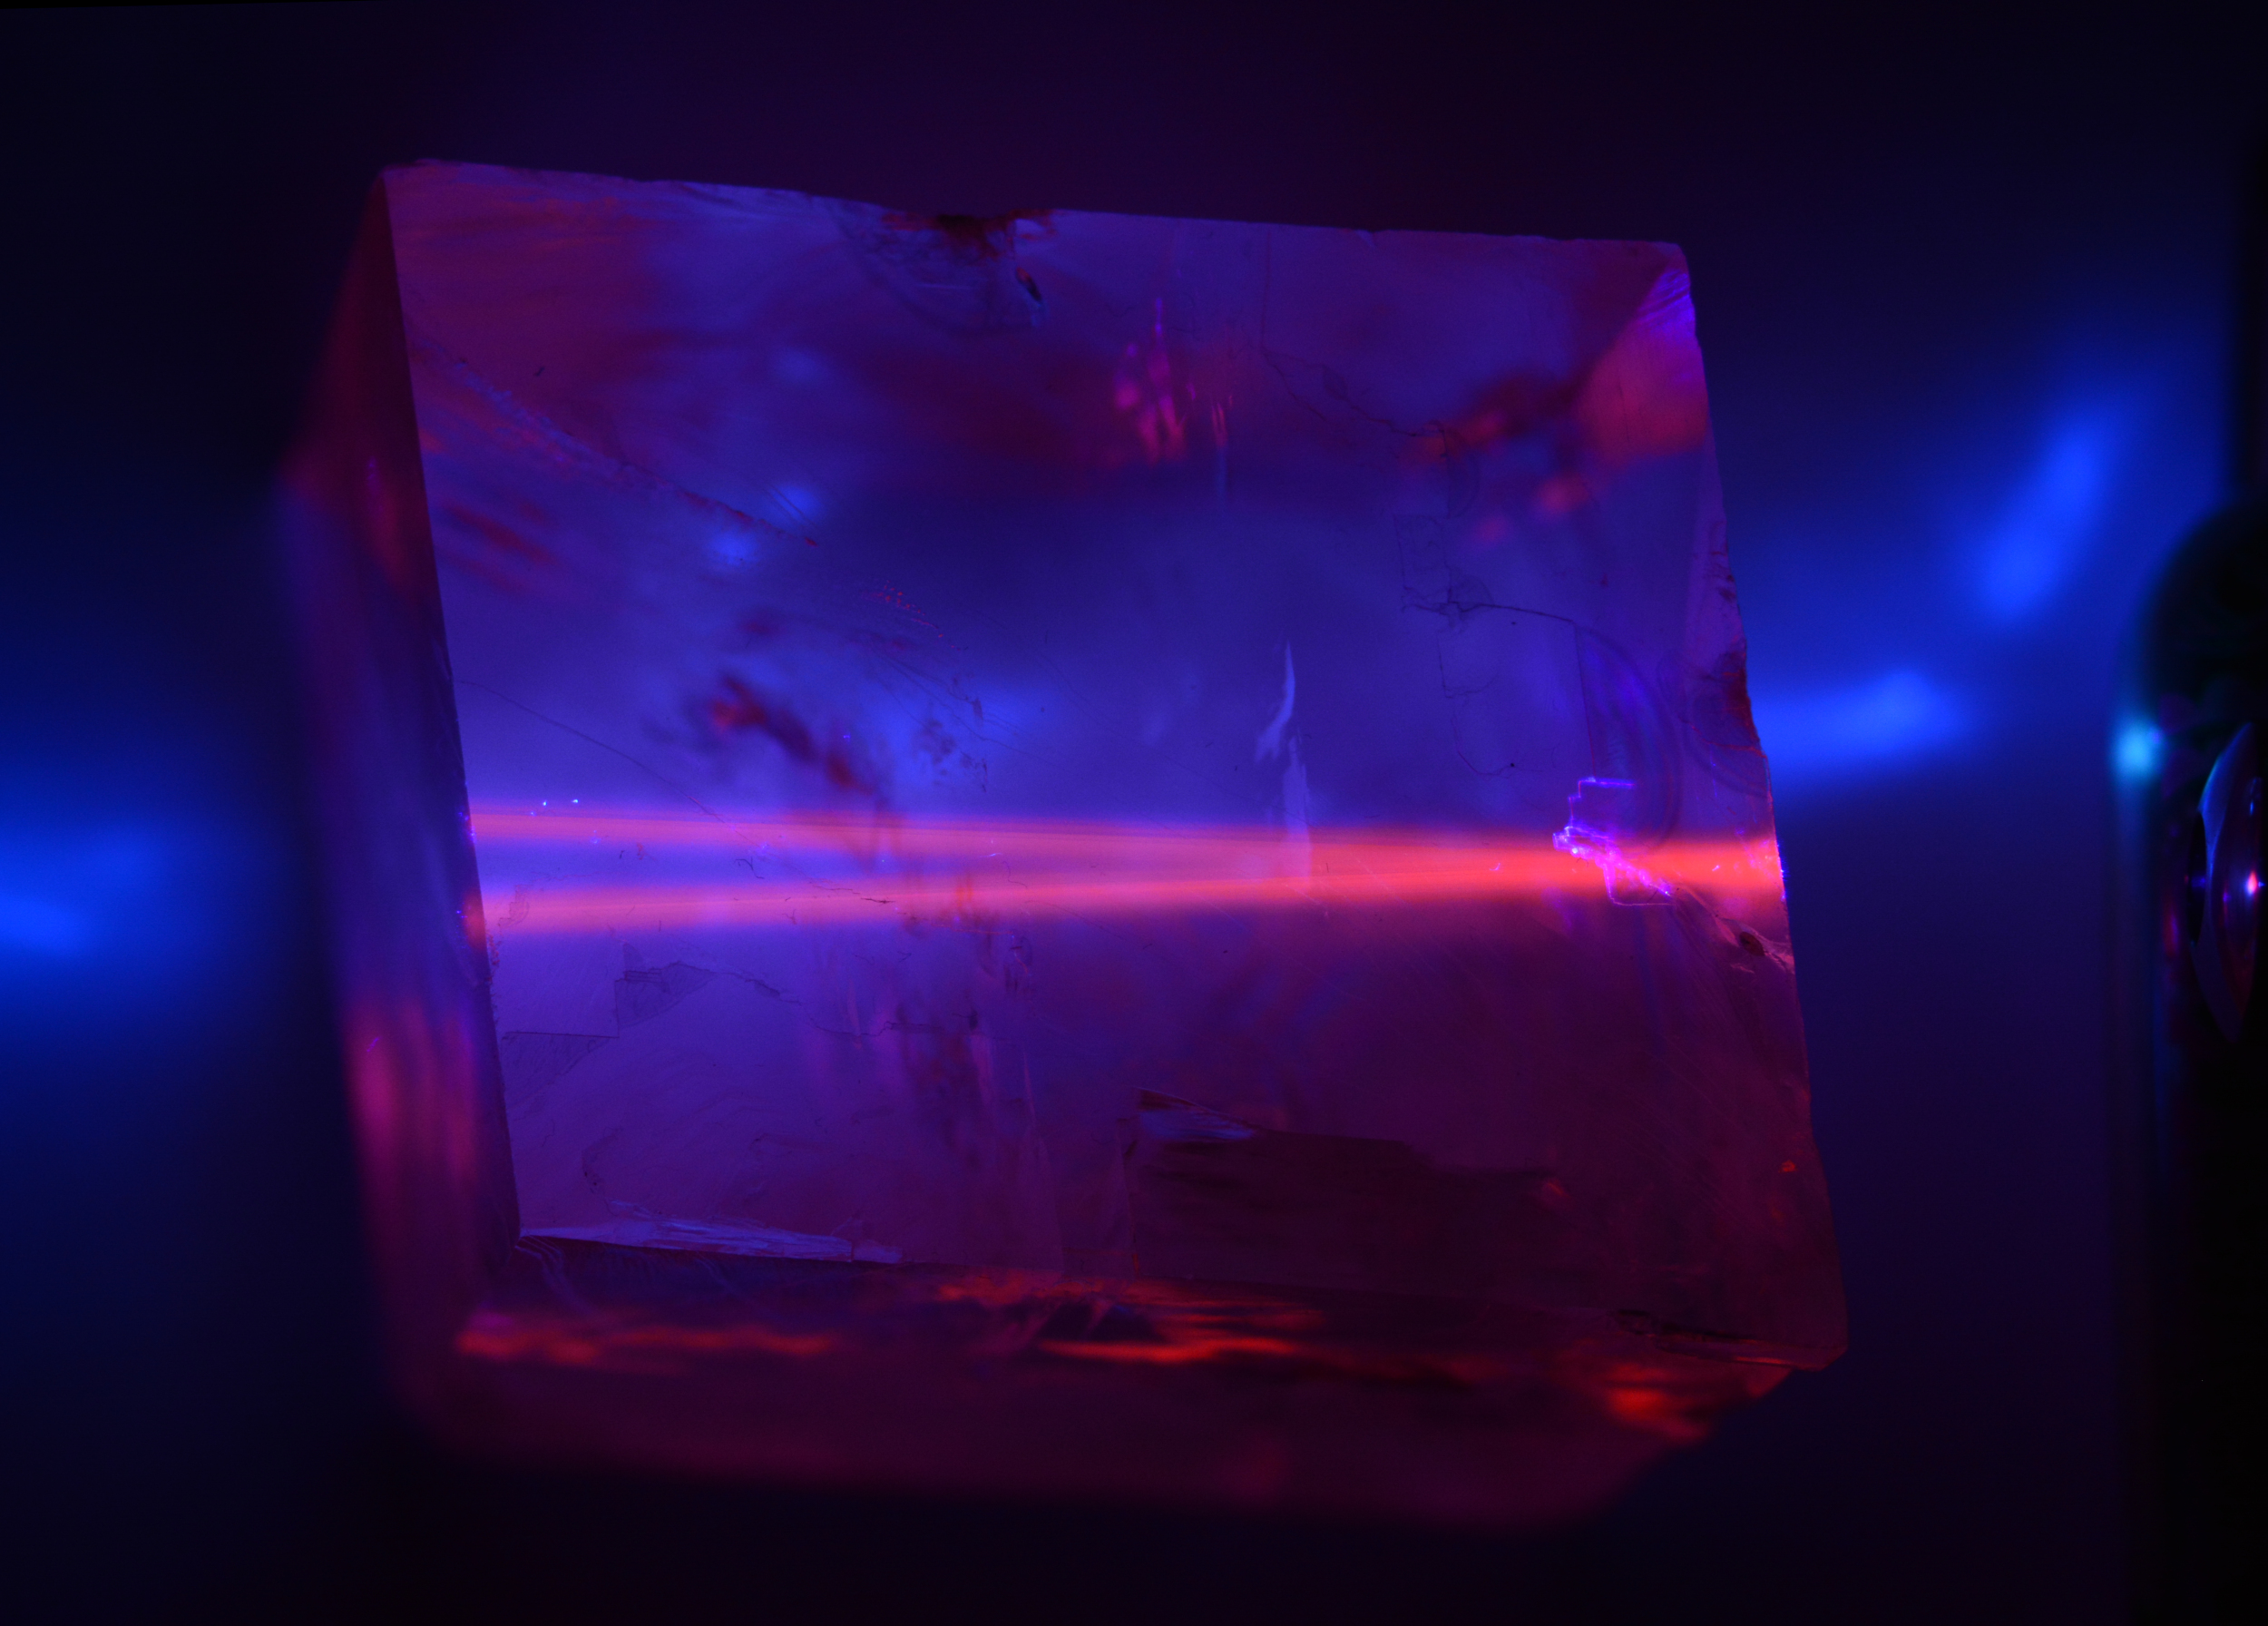
\includegraphics[width=9truecm]{slike/10_FotoDvolom2.jpg}
\caption{Snop svetlobe se pri lomu v kalcit razcepi v dva snopa. Pot svetlobe skozi 
kristal je vidna zaradi fluorescence.}
\label{fig:10_dvolom_2}
\end{figure}
\begin{figure}[h!]
\centering
\def\svgwidth{140truemm} 
\input{slike/10_FotoDvolom.pdf_tex}
\caption{Pri prehodu svetlobe skozi kalcit nastaneta dve sliki, ki sta razmaknjeni (levo). 
Z linearnim polarizatorjem pokažemo, da imata sliki različni polarizaciji (sredina in desno). 
Kalcitu zaradi te optične lastnosti rečemo tudi islandski dvolomec.
}
\label{fig:10_dvolom_2}
\end{figure}

Ko enkrat določimo smeri valovnih vektorjev v snovi, lahko izračunamo tudi 
smeri Poyntingovih vektorjev, ki predstavljajo smer širjenja energije. Za redni 
žarek je račun preprost, saj je Poyntingov vektor vzporeden valovnemu vektorju, za 
izredni žarek pa smer Poyntingovega vektorja odstopa od smeri valovnega vektorja, pri 
čemer je kot med njima enak kotu med smerjo jakosti in smerjo gostote električnega polja. 
Poglejmo nekaj zanimivejših primerov.

\begin{example}{\bf Dvojni lom pri poševnem vpadu na optično enoosno snov.}
Oglejmo si lom svetlobe pri poševnem vpadu na optično enoosno snov, pri katerem 
je optična os vzporedna z mejo med snovema (slika~\ref{fig:10_dvolom_6}). Vpadna
svetloba naj bo nepolarizirana.
\begin{figure}[h]
\centering
\def\svgwidth{140truemm} 
\input{slike/10_dvolom_6.pdf_tex}
\caption{Dvojni lom pri poševnem vpadu nepolarizirane svetlobe iz izotropne v 
optično anizotropno snov, če je optična os vzporedna mejni ravnini: 
dvojni lom v pozitivno anizotropno snov (a) in lom v negativno 
anizotropno snov (b). V obeh primerih 
se vpadni žarek razcepi v dva žarka, ki sta medsebojno ortogonalno polarizirana. Smer 
Poyntingovega vektorja za redni žarek ni prikazana, saj je enaka smeri valovnega vektorja
$\mathbf{k}_r$.}
\label{fig:10_dvolom_6}
\end{figure}

Vemo, da je redni žarek tisti, ki je polariziran pravokotno na 
vpadno ravnino (transverzalno električno oziroma TE valovanje). 
Zanj velja navadni lomni zakon, pri čemer je lomni količnik v snovi 
redni lomni količnik $n_r$ (enačba~\ref{eq:rednilom}). Velja:
\beq
n_0 \sin\alpha = n_r \sin \beta_r = \sqrt{\varepsilon_\perp}\sin\beta_r.
\label{eq:10_110}
\eeq
Pri tem smo z $\alpha$ označili vpadni kot, z $\beta_r$ pa lomni kot rednega žarka.

Po drugi strani transverzalna magnetna (TM) komponenta vpadne svetlobe, pri kateri
polarizacija leži v vpadni ravnini, predstavlja tisti del, ki se lomi
kot izredni žarek z lomnim količnikom $n_i$ (enačba~\ref{eq:izrednilom}). Zanj velja:
\beq
n_0 \sin \alpha = n_i \sin\beta_i,
\label{eq:10_111}
\eeq
pri čemer $\beta_i$ označuje lomni kot izrednega žarka glede na normalo na mejno ravnino.
Ne smemo pozabiti, da v enačbah za izračun lomnega količnika v odvisnosti od smeri 
valovnega vektorja (enačba~\ref{eq:izredni}) nastopa kot $\vartheta$ glede na smer optične osi.
Med kotoma $\beta_i$ in $\vartheta$ zato v opisanem primeru velja zveza:
\beq
\beta_i + \vartheta = \pi/2.
\label{eq:10_112}
\eeq
Lomni količnik pri kotu $\beta_i$ potem izračunamo iz enačbe~(\ref{eq:izredni}):
\beq
\frac{1}{n_i^2} = \frac{\sin^2(\pi/2-\beta_i)}{n_\myparallel^2} + 
\frac{\cos^2(\pi/2-\beta_i)}{n_\perp^2} = 
\frac{\cos^2\beta_i}{n_\myparallel^2} + 
\frac{\sin^2\beta_i}{n_\perp^2},
\label{eq:10_113}
\eeq
od koder sledi:
\beq
n_i = \frac{1}{\sqrt{\cos^2\beta_i/n_\myparallel^2 + 
\sin^2\beta_i/n_\perp^2}}.
\label{eq:10_114}
\eeq
Vstavimo izraz za lomni količnik v lomni zakon (enačba~\ref{eq:10_111}) in ga kvadriramo:
\beq
n_0^2 \sin^2\alpha \left(\frac{\cos^2\beta_i}{n_\myparallel^2} + 
\frac{\sin^2\beta_i}{n_\perp^2}\right) = \sin^2\beta_i.
\label{eq:10_115}
\eeq
Z uporabo zveze med kotnimi funkcijami $\cos^2\varphi = 1 - \sin^2 \varphi$ dobimo:
\beq
\sin^2\beta_i = 
\frac{n_0^2 \sin^2\alpha}{n_\myparallel^2} + 
\left(\frac{n_0^2 \sin^2\alpha}{n_\perp^2} - \frac{n_0^2 \sin^2\alpha}{n_\myparallel^2}
\right)\sin^2\beta_i.
\label{eq:10_116}
\eeq
Sledi:
\beq
\sin\beta_i = \frac{n_0 \sin \alpha}{\sqrt{n_\myparallel^2 - \left(n_\myparallel^2
/n_\perp^2 -1\right)n_0^2 \sin^2\alpha}}.
\label{eq:10_117}
\eeq
Enačbi~(\ref{eq:10_110} in \ref{eq:10_117}) uporabimo za izračun lomnega kota, ki podaja 
smer valovnega vektorja v snovi. Za izračun smeri prenosa energije oziroma smeri 
Poyntingovega vektorja moramo upoštevati tudi, da smeri $\mathbf{k}$ in $\mathbf{S}$
za izredni žarek nista vzporedni. Kot med njima $\gamma$ izračunamo z enačbo~(\ref{eq:10_105}),
pri čemer moramo upoštevati razliko med lomnim kotom $\beta_i$ in kotom $\vartheta$,
ki nastopa v enačbi za elipso ~(\ref{eq:10_112}).

Za kristale z negativno optično anizotropijo (slika~\ref{fig:10_dvolom_6}\,) je račun zelo 
podoben. Razlika nastanek pri izračunu smeri Poyntingovega vektorja, saj se 
pri negativno anizotropnih snoveh kot $\gamma$ (kot med $\mathbf{k}$ in $\mathbf{S}$)
odšteje od lomnega kota $\beta_i$, pri pozitivno anizotropnih pa prišteje.
\end{example}

%%%%%%%%%%
\begin{example}{\bf Dvojni lom pri pravokotnem vpadu.}
\label{chap:dvolomfaza}
Obravnavajmo poseben primer prejšnjega zgleda, ko svetloba vpada pravokotno na mejo
med izotropno in anizotropno snovjo, optična os pa naj bo še vedno vzporedna z mejo 
med snovema (slika~\ref{fig:10_dvolom_3}).
\begin{figure}[h]
\centering
\def\svgwidth{140truemm} 
\input{slike/10_dvolom_3.pdf_tex}
\caption{Pravokotni vpad svetlobe iz izotropne v optično anizotropno snov vzdolž 
lastne osi}
\label{fig:10_dvolom_3}
\end{figure}

Redni žarek se po pričakovanju ne lomi in tako valovni kot Poyntingov vektor kažeta
v smeri pravokotno na mejno ravnino. Pri izrednem žarku je podobno, saj je smer
valovnega vektorja v smeri normale, s slike pa vidimo, da je tudi
smer Poyntingovega vektorja (normala na elipso) vzporedna z valovnim vektorjem. 
Redni in izredni žarek zato v tem primeru potujeta v isti smeri in po prehodu 
iz kristala izstopata na istem mestu. Ker pa se različni polarizaciji širita z različnima
hitrostma, med njima nastane fazna razlika, ki je odvisna od debeline snovi $L$. 
Fazno razliko med izrednim in rednim žarkom zapišemo kot:
\beq
\Delta \phi = \phi_i-\phi_r = k_0 L (n_i-n_r) = k_0 L (n_\myparallel - n_\perp).
\label{eq:10_108}
\eeq
Če na snov posvetimo z linearno polarizirano svetlobo, katere polarizacija se ne ujema
z lastnimi osmi snovi, tako med posameznima komponentama vpadne polarizacije nastane
fazni zamik. S spreminjanjem debeline snovi lahko spreminjamo zamik $\Delta \phi$,
kar uporabljamo za izdelavo retardacijskih ploščic (glej razdelek~\ref{chap:komponente}).
Kadar se polarizacija vpadne svetlobe ujema z eno od lastnih osi snovi, se ohranjata 
tako polarizacija kot smer širjenja svetlobe.
\end{example}

\begin{example}{\bf Dvojni lom pri pravokotnem vpadu in splošni smeri optične osi.}
Za konec poglejmo še pravokotni vpad na optično enoosno snov, v kateri je optična os
nagnjena glede na mejno ravnino. 
\begin{figure}[!h]
\centering
\def\svgwidth{140truemm} 
\input{slike/10_dvolom_7.pdf_tex}
\caption{Pravokotni vpad svetlobe na optično anizotropno snov z nagnjeno optično osjo}
\label{fig:10_dvolom_7}
\vglue-3truemm
\end{figure}

Pri pravokotnem vpadu se smer valovnega vektorja ohranja tako za redni kot za izredni 
žarek. Za redni žarek je smer Poyntingovega vektorja vzporedna valovnemu vektorju, 
tako da žarek tudi v snovi potuje v smeri normale. 
Poyntingov vektor za izredni žarek pa je v smeri tangentno na elipso in zato 
nagnjen za kot $\gamma$ glede na normalo na mejno ploskev. Po vpadu na  optično 
anizotropno snov z nagnjeno optično osjo tako tudi pri pravokotnem vpadu svetlobe 
pride do loma, pri čemer se lomi valovanje s TM polarizacijo, TE polarizirano 
valovanje pa ne. Iz snovi izstopata dva različno polarizirana vzporedna žarka, 
zato lahko tako postavitev uporabimo kot polarizator za pridobivanje
linearno polarizirane svetlobe.
\end{example}

\begin{example}{\bf Optično anizotropna snov med prekrižanima polarizatorjema.}
Fazni zamik med polarizacijama pri prehodu skozi optično anizotropno snov je 
odvisen tudi od valovne dolžine svetlobe (enačba~\ref{eq:10_108}). 
Polarizacija valovanj z različnimi valovnimi dolžinami se zato v snovi zasuče za različne kote 
in če anizotropno snov postavimo med prekrižana polarizatorja, bodo nekatere barve bolj prepuščene
od drugih, nekatere pa sploh ne. Snov zato na splošno vidimo obarvano 
(slike~\ref{fig:10_nematik} in \ref{fig:10_dvolom_5}).
\begin{figure}[ht]
\centering
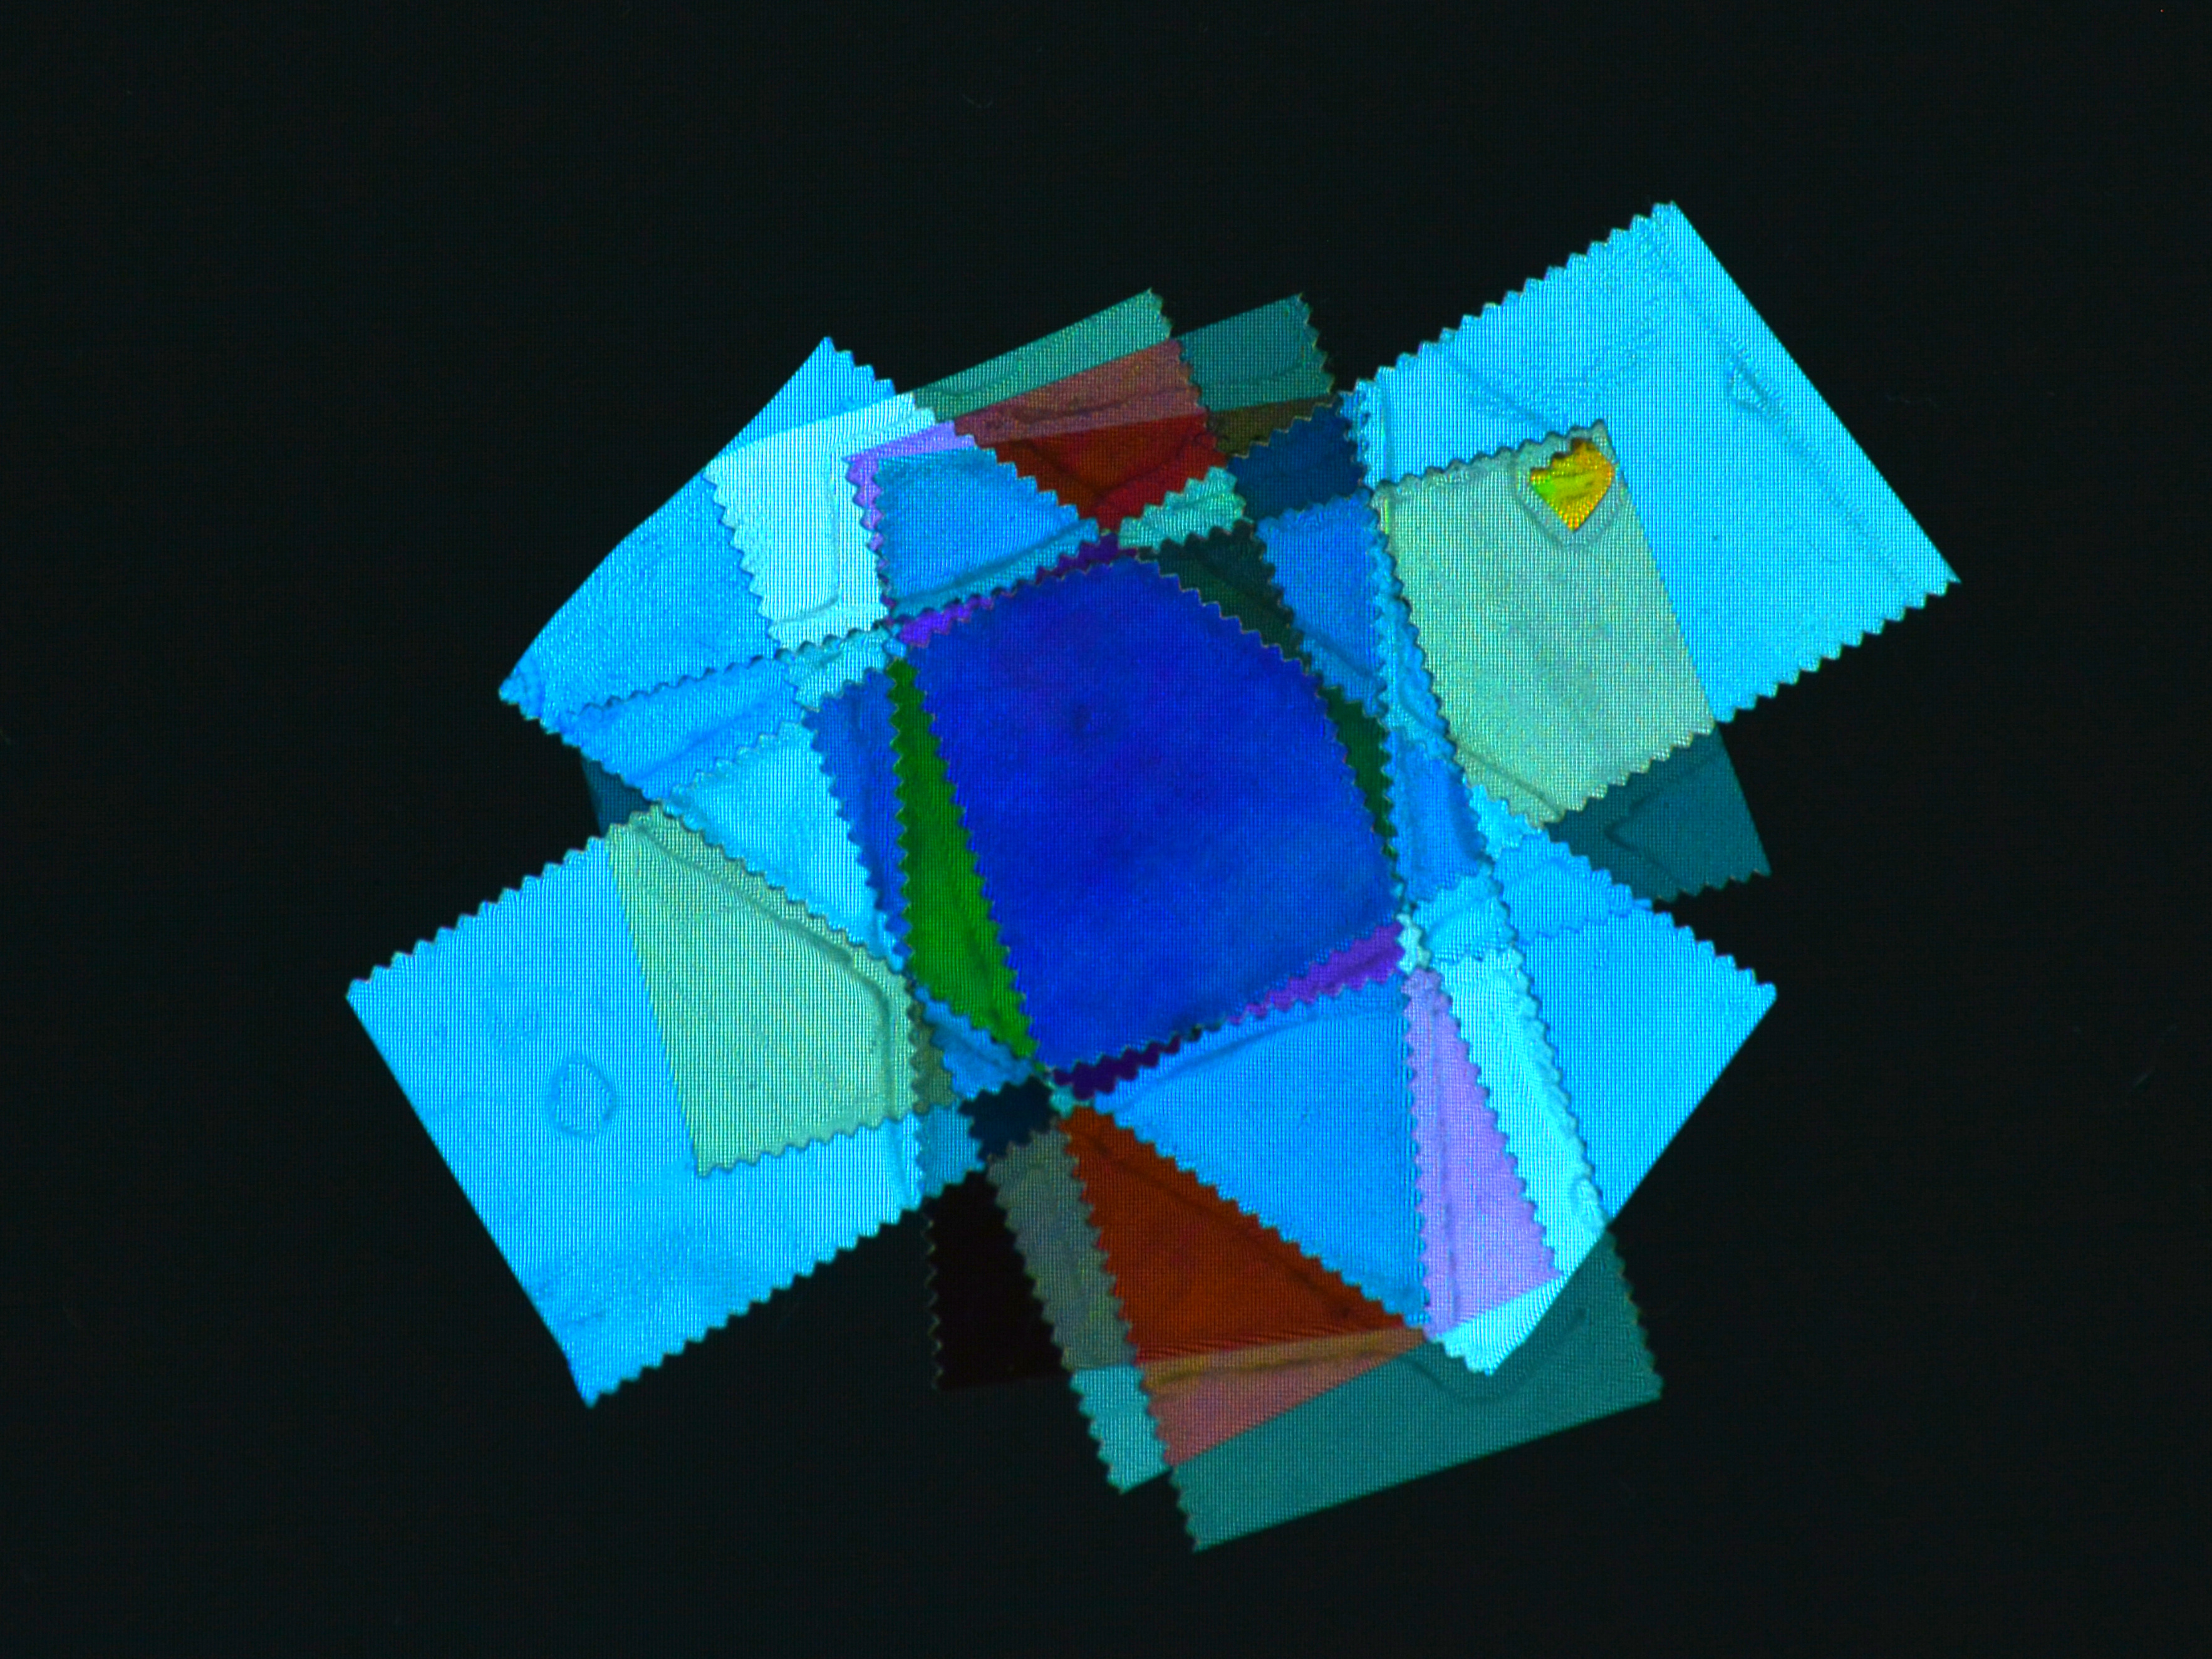
\includegraphics[width=7truecm]{slike/10_FotoDvolom5a.jpg}\hfill
\includegraphics[width=7truecm]{slike/10_FotoDvolom5b.jpg}
\caption{Primer optično anizotropne snovi je lepilni trak. Kadar naključno zlepimo več 
plasti, so fazni zamiki na različno debelih in različno orientiranih delih različni. 
Svetloba, prepuščena skozi analizator, je zato različnih barv (a). Ko analizator sučemo, 
se barve vzorca spreminjajo~(b).}
\label{fig:10_dvolom_5}
\end{figure}
\vglue-3truemm
\end{example}

\section{Optične komponente na osnovi dvolomnih snovi}
\label{chap:komponente}
Dodobra smo spoznali širjenje snovi v optično anizotropnih snoveh in spoznali dvojni lom.
Poglejmo zdaj načine uporabe dvojnega loma in optične komponente na osnovi dvolomnih snovi.
Večinoma so to optične komponente, s katerimi učinkujemo na polarizacijo
svetlobe, oziroma naprave, ki se odzivajo na vpadno elektromagnetno valovanje v odvisnosti
od njegove polarizacije.

\subsection*{Polarizatorji}
Ker se po prehodu skozi dvolomno snov redni in izredni žarek na splošno razmakneta, 
lahko dvolomne snovi uporabimo za pridobivanje linearno polarizirane svetlobe iz nepolarizirane
vpadne. Dvolomne snovi tako lahko delujejo kot polarizatorji.

Prvi primer je Nicolova prizma, ki jo imenujemo po škotskem geologu in fiziku
Williamu Nicolu (1770--1851). Nicolova prizma je navadno sestavljena iz dveh kalcitnih prizem, ki 
sta med seboj zlepljeni (slika~\ref{fig:10_Nicol}) s kanadskim balzamom\footnote{Kanadski balzam je neke vrste 
terpentin, pridobljen iz smole balzamovca, iglavca iz rodu jelk.}. 
Lomni količnik kanadskega balzama $n_0=1,550$ in velja:
\beq
n_\perp = 1,658 > n_0 = 1,550 > n_\myparallel = 1,486.
\label{eq:10_119}
\eeq
Pri tem sta $n_\perp$ in $n_\myparallel$ lastna lomna količnika kalcita. 
Prizmi sta odrezani pod takim kotom ($\approx 68\si{\degree}$), da se ena polarizacija na 
meji z lepilom totalno odbije. Ker je kalcit negativno anizotropen, se totalno odbije redno polarizirani
žarek. Izredni žarek je skoraj v celoti prepuščen, saj je vpadni kot blizu Brewstrovega kota in je zato
odbojnost za TM polarizacijo zelo majhna. Na izhodu iz prizme v smeri naprej dobimo 
TM linearno polarizirano valovanje.
\vglue3truemm
\begin{figure}[!h]
\centering
\def\svgwidth{130truemm} 
\input{slike/10_Nicol.pdf_tex}
\caption{Nicolova (a) in Wollastonova prizma (b) delujeta kot polarizatorja.}
\label{fig:10_Nicol}
\end{figure}

Drugi primer je Wollastonova prizma, imenovana po angleškem kemiku in fiziku 
Williamu Hyde Wollastonu (1766--1828). Prizma je sestavljena iz dveh zlepljenih pravokotnih prizem, 
pri čemer je optična os v drugi prizmi pravokotna glede na optično os v prvi prizmi. 
Na meji med prizmama se valovanje razdeli na dve linearno polarizirani komponenti, 
ki zapustita prizmo vsaka v svoji smeri. 

\begin{remark}
Poleg omenjenih prizem poznamo veliko drugih polarizacijskih prizem. Na totalnem odboju temeljijo
poleg Nicolove prizme še na primer Glan-Taylorjeva prizma (sestavljena iz dveh pravokotnih prizem, 
med katerima je zračna reža, optični osi prizem pa ležita v ravnini osnovne ploskve prizme vzporedno 
z vpadno stranico), Glan-Thompsonova prizma (sestavljena iz dveh zlepljenih pravokotnih prizem, 
optični osi prizem pa sta pravokotni na osnovni ploskvi prizme) in Glan-Foucaulteva prizma 
(podobna kot Glan-Thompsonova, le da je med prizmama zračna reža). Paul Glan (1846--1898), 
po katerem se te prizme imenujejo, je bil nemški fizik in meteorolog. Na razklonu žarkov
pa poleg Wollastonove prizme delujejo med drugimi Nomarskijeva prizma (dve zlepljeni pravokotni prizmi, 
optična os prve leži v ravnini osnovne ploskve, druge pa je pravokotna nanjo), Rochonova prizma
(podobna Nomarskijevi, le da je optična os prve prizme vzdolž vpadne svetlobe) in 
S\'enarmontova prizma (podoba Normanskijevi, le da je optična os prve prizme vzporedna vpadni svetlobi).
\end{remark}

\subsection*{Retardacijske ploščice}
Kadar svetloba vpada pravokotno na anizotropno snov vzdolž lastne osi kristala 
(glej primer~\ref{chap:dvolomfaza}) se redni in 
izredni žarek širita v isti smeri, med njima pa nastane fazni zamik oziroma retardacija, če se le 
ne širita vzdolž optične osi.
Ploščice, ki med dvema ortogonalnima komponentama vpadne polarizacije ustvarijo
fazni zamik, imenujemo retardacijske ploščice. Njihov učinek opišemo z Jonesovo matriko:
\beq
M = 
\left[\begin{array}{cc}
e^{-i\Delta \phi/2} & 0\\
0 & e^{i\Delta \phi/2}\\
\end{array}\right]\!\!.
\label{eq:10_120}
\eeq
Pri tem je $\Delta \phi = k_0 L (n_i-n_r)$, kjer je $L$ dolžina kristala, $n_i$ in $n_r$
pa označujeta redni in izredni lomni količnik snovi (enačba~\ref{eq:10_108}). 
Če je $\Delta \phi= \pi/2$, retardacijski ploščici pravimo ploščica $\lambda/4$. 
Ploščica $\lambda/4$ iz linearne polarizacije naredi cirkularno polarizirano svetlobo. 
Kadar je fazni zamik $\pi$, element deluje kot ploščica $\lambda/2$, ki spremeni smer
krožno polariziranega valovanja oziroma zasuče smer linearno polariziranega valovanja.

\subsection*{Kompenzatorji}
Slabost retardacijskih ploščic je v tem, da imajo izbrano retardacijo le za 
točno določeno valovno dolžino. Če želimo narediti element, ki je uporaben za svetlobo z 
različnimi valovnimi dolžinami, uporabimo tako imenovani kompenzator. Z njim lahko 
ustvarimo poljubni fazni zamik med ortogonalnima polarizacijama. 
\begin{figure}[!h]
\centering
\def\svgwidth{80truemm} 
\input{slike/10_Soleil.pdf_tex}
\caption{Babinet-Soleilev kompenzator. S premikanjem klinaste ploščice spreminjamo
fazni zamik med ortogonalnima komponentama polarizacije prepuščene svetlobe.}
\label{fig:10_Soleil}
\end{figure}

Primer kompenzatorjev je Babinet-Soleilev kompenzator.
Sestavljen je iz treh elementov iz iste snovi: ene planparalelne ploščice in dveh klinastih ploščic, 
pri čemer je optična os v ploščici pravokotna na optični osi v klinastih ploščicah 
(slika~\ref{fig:10_Soleil}). S pomikanjem klinaste ploščice v smeri pravokotno na smer vpadne 
svetlobe lahko poljubno nastavljamo fazni zamik (retardacijo) med obema lastnima polarizacijama.

Če označimo debelino planparalelne ploščice z $L_1$ in skupno debelino obeh klinastih ploščic
na mestu vpadne svetlobe $L_2$, potem je fazni zamik med polarizacijama po prehodu skozi kompenzator
enak:
\beq
\Delta \phi = k_0 (L_1 - L_2) (n_i - n_r).
\eeq
\vglue-3truemm
\begin{remark}
Poleg ploščic $\lambda/4$, ki ustvarijo fazni zamik $\pi/2$, in ploščic $\lambda/2$,
ki ustvarijo fazni zamik $\pi$, so zanimive tudi ploščice $\lambda$. Te na prvi pogled nimajo
posebnega učinka, saj je fazni zamik, ki ga dodajo valovanju, enak $2\pi$. Vendar je ta zamik odvisen
od valovne dolžine in je enak $2\pi$ le pri točno določeni valovni dolžini,
za vse ostale pa je izhodna polarizacija na splošno eliptična. Če na izhod dodamo 
analizator, taka ploščica izloči le izbrano valovno dolžino, ostale pa vsaj delno prepusti. 
Navadno se uporablja ploščico za valovno dolžino $\sim 540~\si{nm}$, zato so med prekrižanima
polarizatorjema videti izrazito rožnato. Uporablja se jih pri mikroskopiji za določanje predznaka
optične anizotropije in povečanje kontrasta. Med vzporednima polarizatorjema jih uporabljamo
v optičnih sistemih za odpravljanje morebitnih neželenih sprememb linearne polarizacije. 
\end{remark}

\section{Konoskopija}
Konoskopija je eksperimentalna metoda za analizo in vizualizacijo optično anizotropnih snovi. 
Navadno želimo izvedeti, ali je snov optično enoosna ali dvoosna, ter določiti orientacijo 
optičnih osi. Z uporabo te metode lahko poleg orientacije optičnih osi določimo 
tudi glavne lomne količnike $n_1$, $n_2$ in $n_3$. Konoskopija je izredno uporabna v mineralogiji
za identifikacijo in določanje lastnosti mineralov.

Princip delovanja je preprost: tanko plast snovi, ki jo proučujemo, postavimo med dva prekrižana 
polarizatorja in jo osvetlimo s koničnim snopom svetlobe. Vpadni žarki, ki na snov vpadajo
pod različnimi vpadnimi koti, se zaradi dvolomnosti razcepijo glede na polarizacijo, nato 
pa se ob izhodu prispevki iz različnih vpadnih žarkov seštejejo v na splošno eliptično valovanje.
Skozi analizator zato ponekod izhaja več svetlobe, ponekod pa manj in na 
opazovalnem zaslonu se pojavijo svetle in temne interferenčne proge, katerih lega in oblika je 
odvisna od dvolomnosti snovi. Ločimo dve vrsti črt na zaslonu: svetle črte imenujemo izokrome, temne
pa izogire. Izokrome nastanejo na mestih, na katerih nastane za dano valovno dolžino $\lambda$ 
fazni zamik $N2\pi$. Kadar osvetljujemo z belo svetlobo, so izokrome črte iste barve, kar da
izokromam tudi ime. Izogire so temne črte in se pojavijo, kadar vpadna
polarizacija ustreza eni od lastnih polarizacij $\mathbf{D}_1$ ali $\mathbf{D}_2$. Iz oblike
opazovanega vzorca hitro določimo, ali je kristal enoosen ali dvoosen in z računom tudi lomne
količnike snovi.
\begin{figure}[ht]
\centering
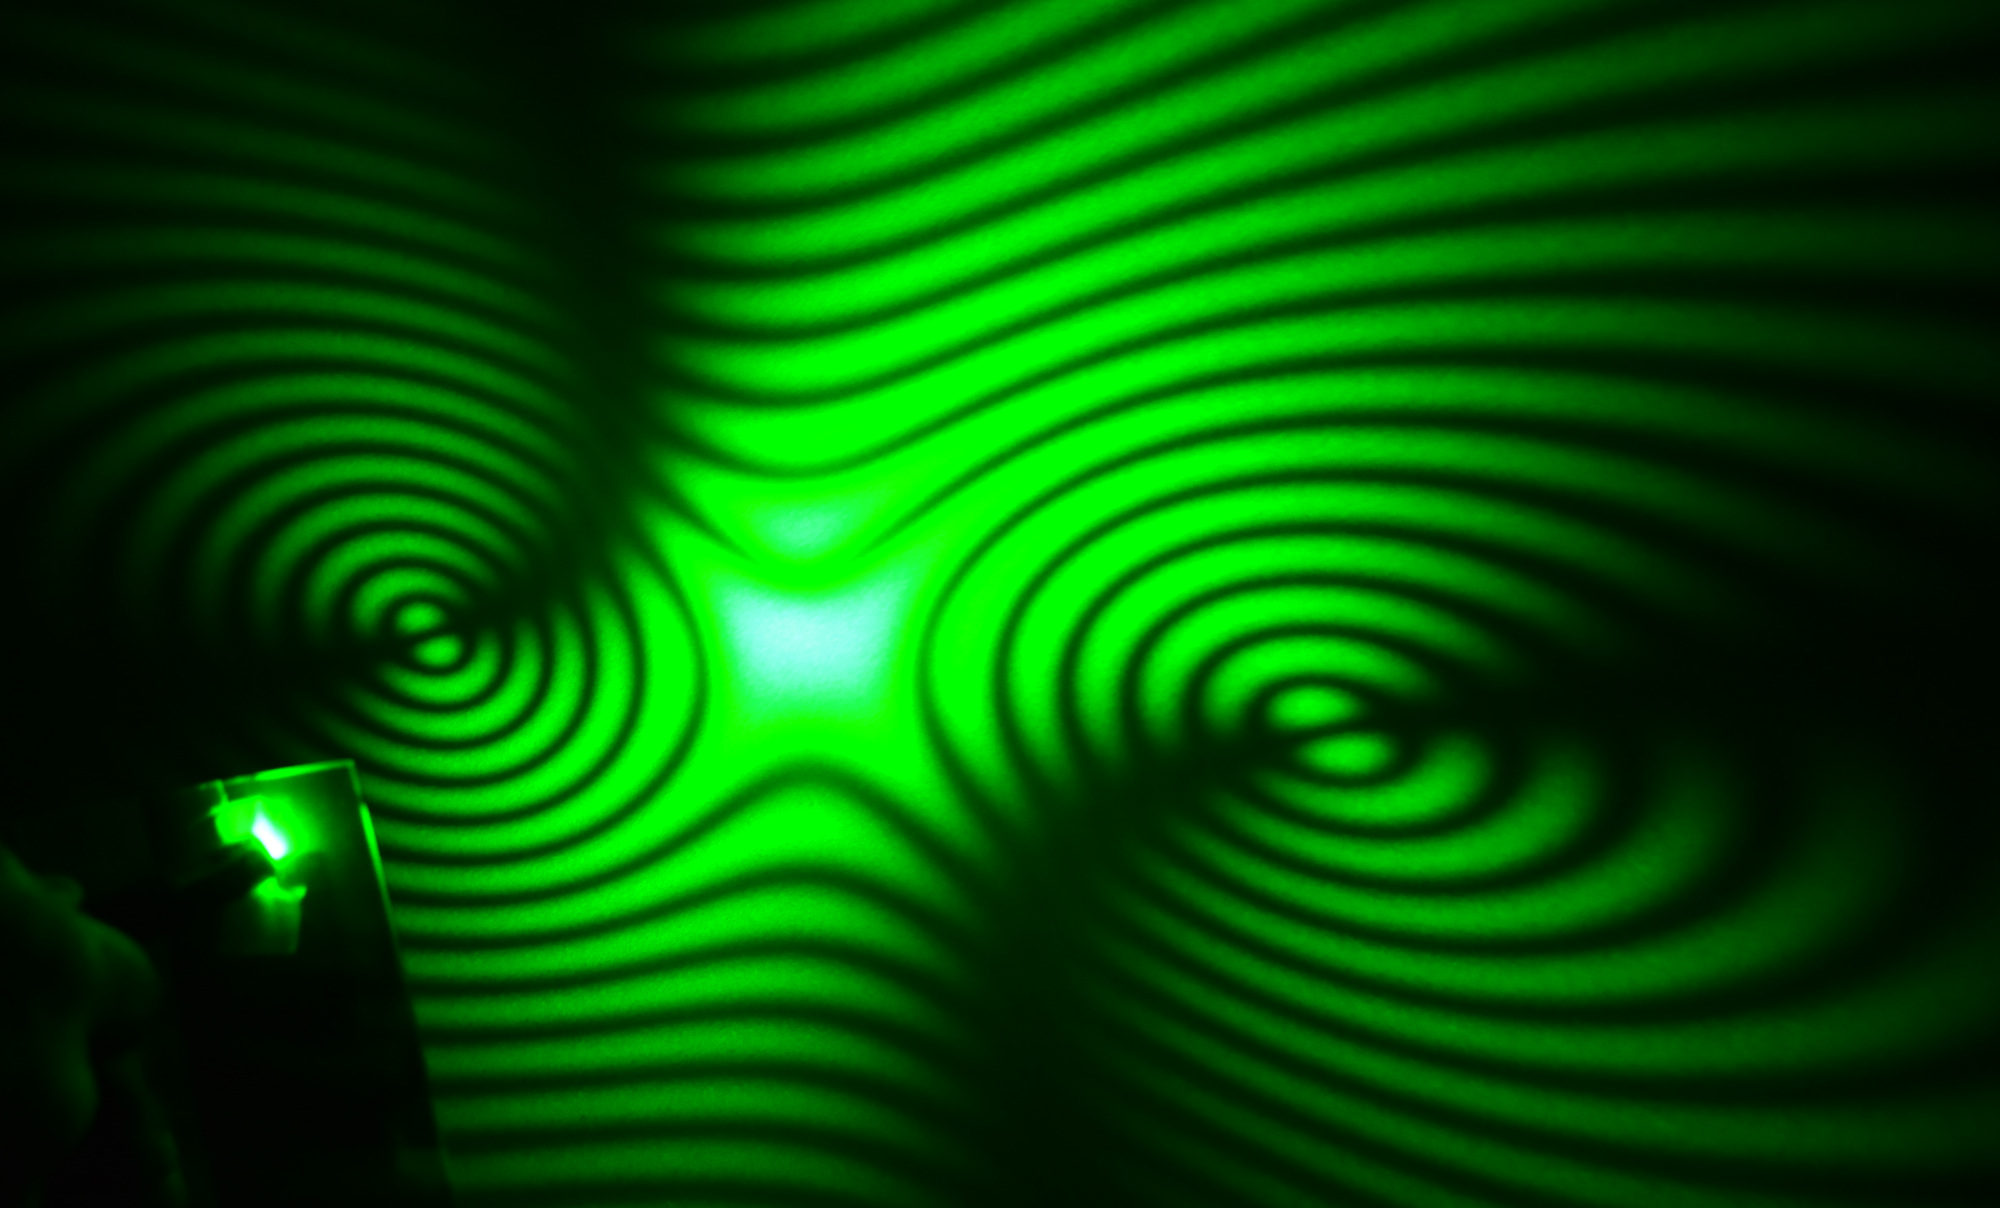
\includegraphics[width=7truecm]{slike/10_Konoskopija1.jpg}\hfill
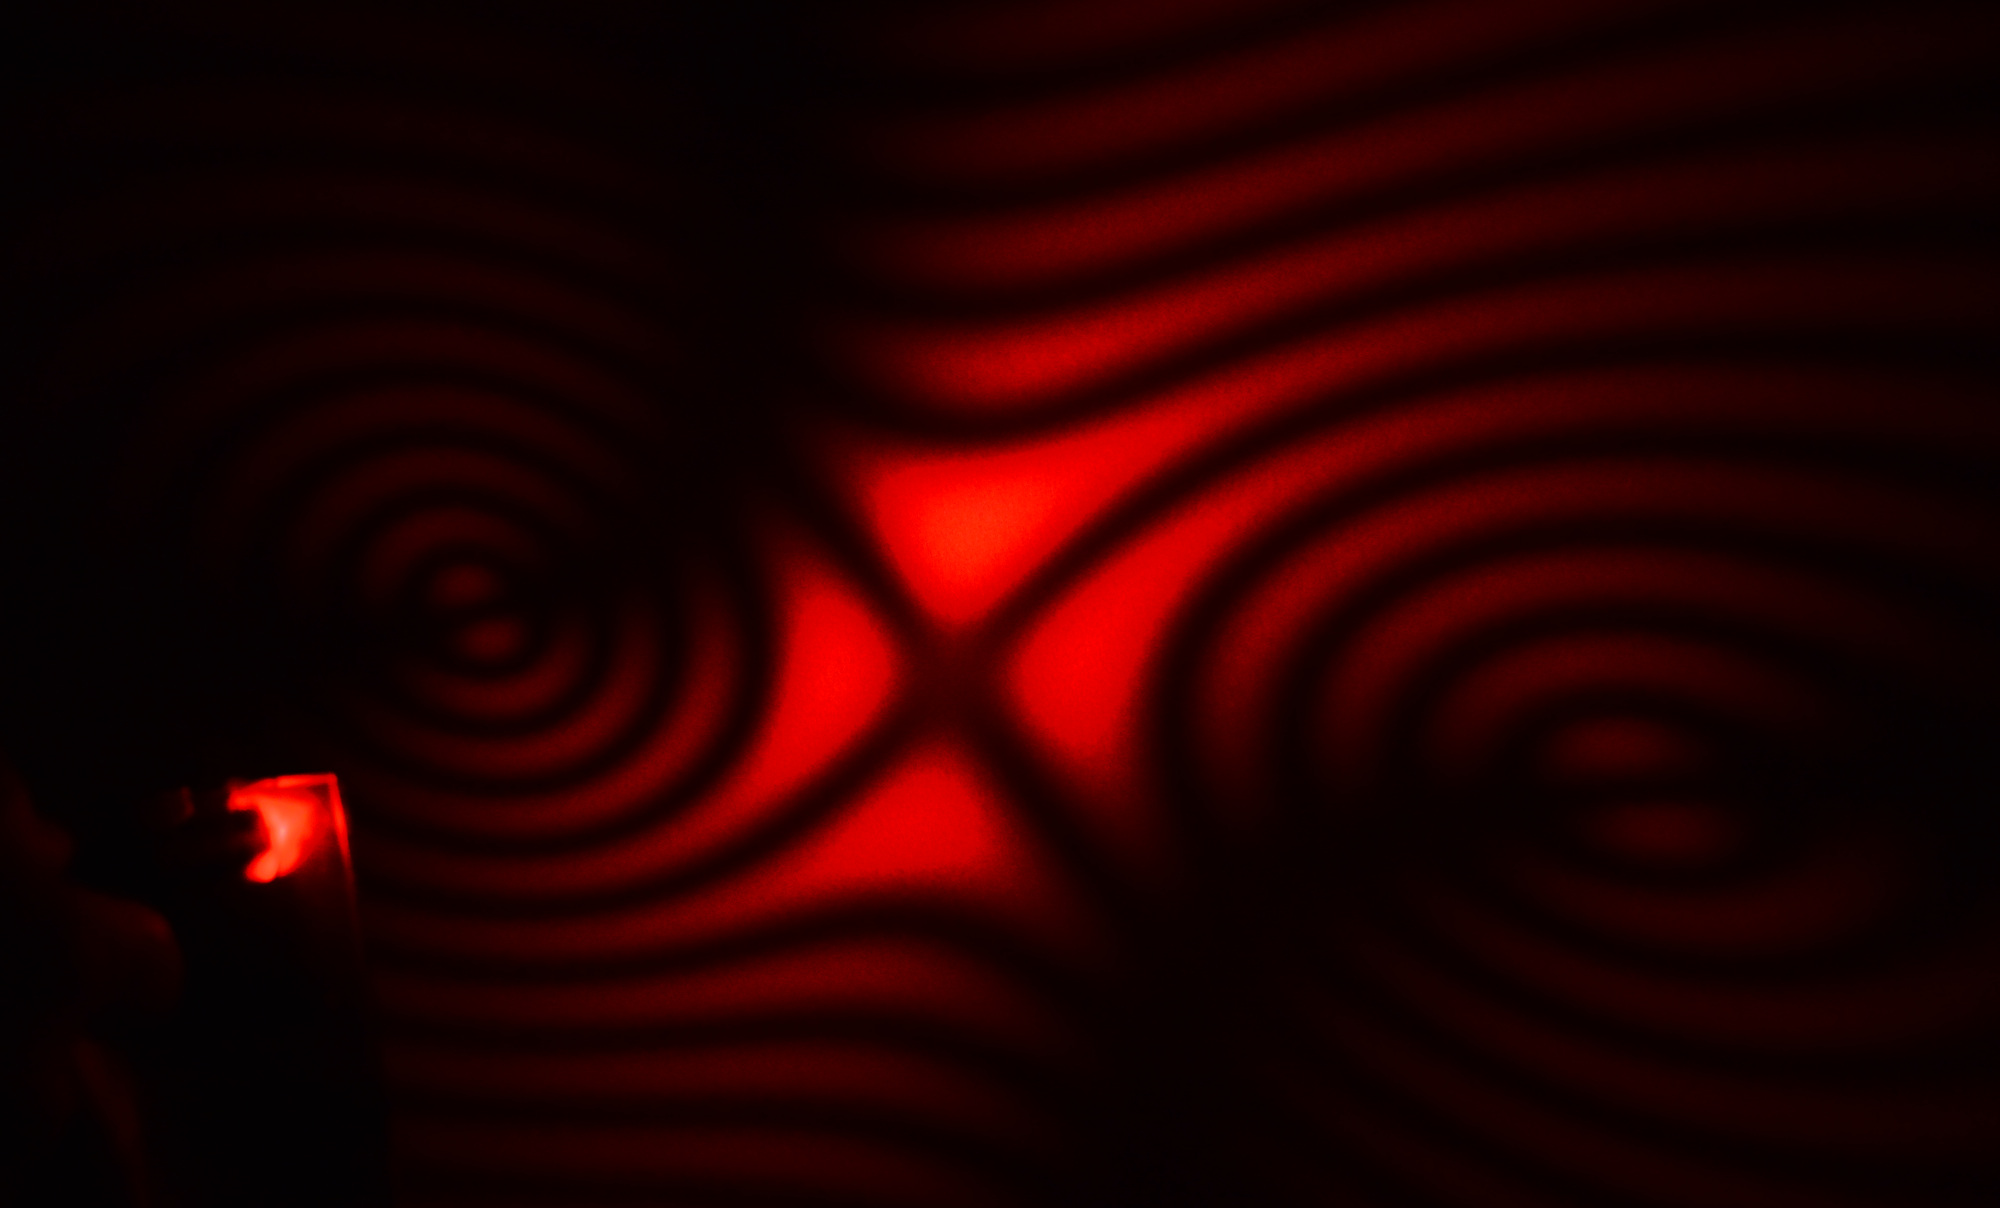
\includegraphics[width=7truecm]{slike/10_Konoskopija2.jpg}
\caption{Poenostavljen konoskopski eksperiment lahko naredimo tudi sami: na izhod laserskega
kazalnika prilepimo moten lepilni trak, s čimer svetlobo razpršimo, in posvetimo na tanko plast
dvolomne snovi med prekrižanima polarizatorjema. Optično dvoosno snov (plastična folija)
prepoznamo po dveh 'očesih' (levo). Vzorec prepuščene svetlobe je odvisen od valovne dolžine (desno).}
\label{fig:10_konoskopija}
\vglue-4truemm
\end{figure}
\begin{figure}[ht]
\centering
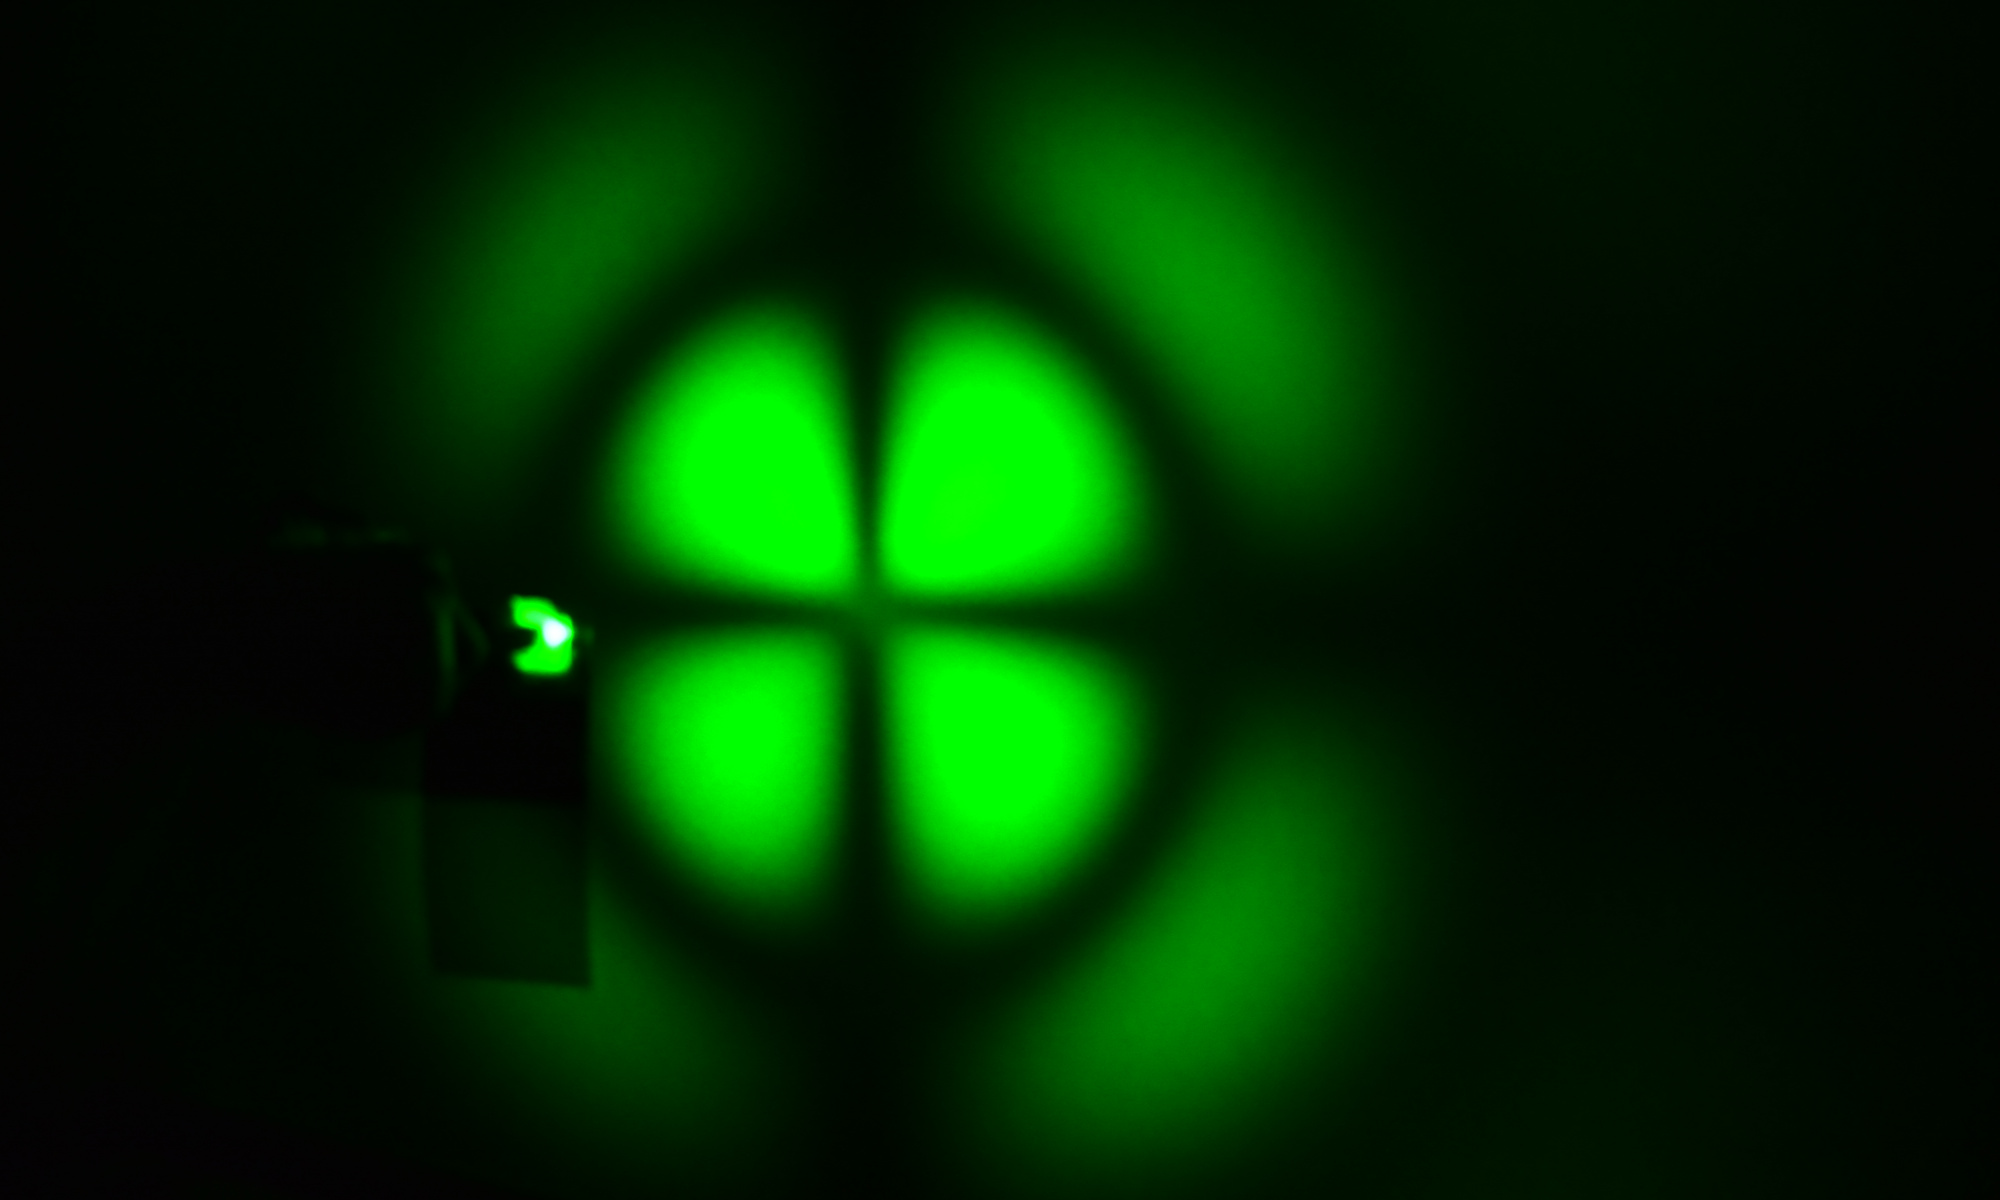
\includegraphics[width=7truecm]{slike/10_Konoskopija3.jpg}\hfill
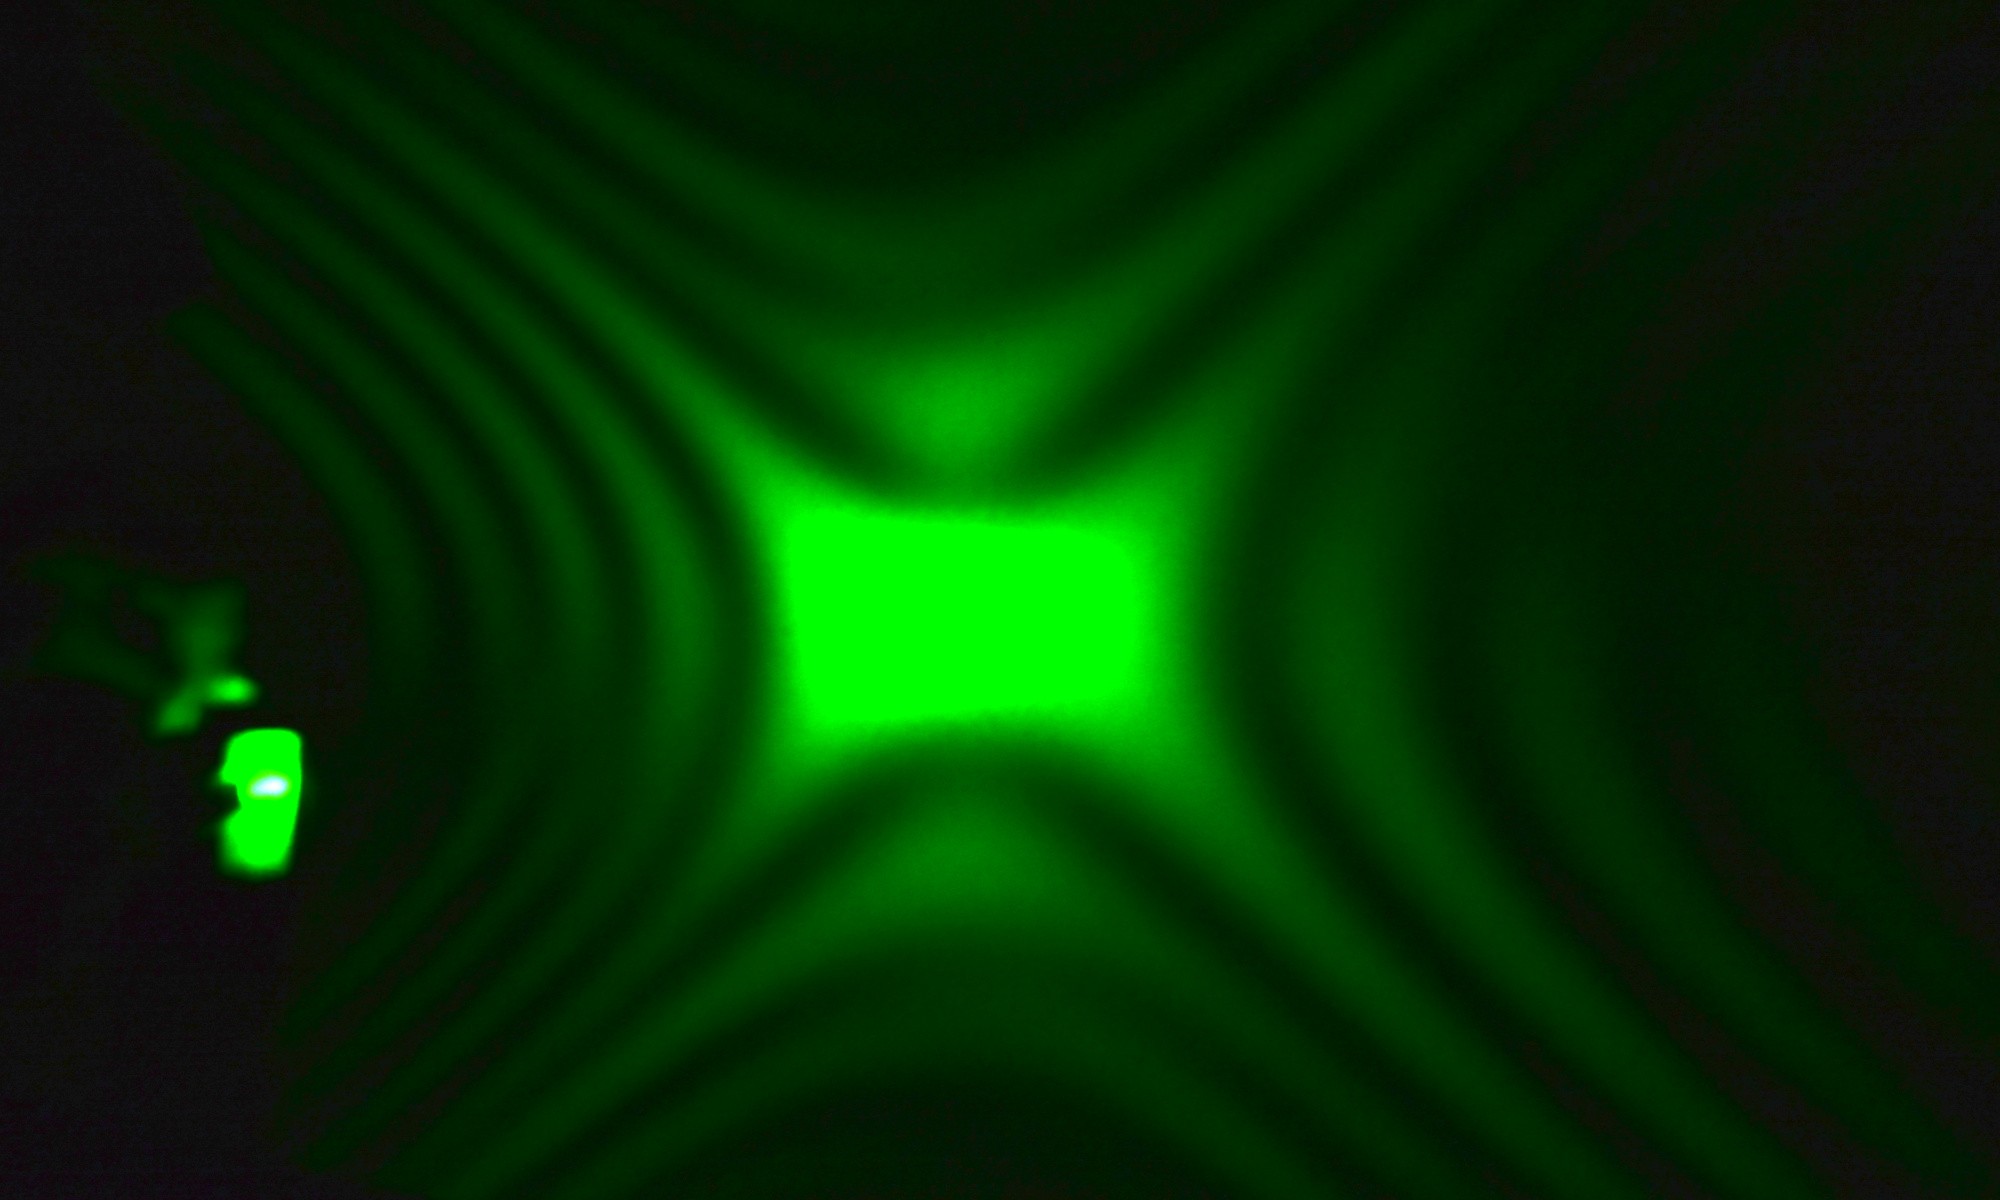
\includegraphics[width=7truecm]{slike/10_Konoskopija4.jpg}
\caption{Konoskopska slika optično enoosne snovi, pri kateri je optična os
pravokotna na polarizatorja (levo) ali vzporedna z njima (desno). Na levi sliki je
tekoči kristal, na desni pa okoli 20 plasti prozornega lepilnega traku.}
\label{fig:10_konoskopija2}
\end{figure}

\end{example}

\section{Inducirana anizotropija}
Do zdaj smo obravnavali naravno dvolomne snovi, katerih dvolomnost je posledica kristalne
strukture ali ureditve anizotropnih molekul. Izkaže se, da lahko dvolomnost umetno
vzpostavimo tudi v sicer optično izotropnih snoveh. Na kratko bomo predstavili dva primera:
optična anizotropija kot posledica mehanske obremenitve ali anizotropija kot posledica
zunanjega električnega polja. 

\subsection*{Fotoelastičnost}
Fotoelastičnost je pojav, pri katerem optično izotropna snov zaradi mehanske obremenitve 
postane optično anizotropna. Ko opazujemo vzorec pod mehansko obremenitvijo med prekrižanima
polarizatorjema, je inducirana dvolomnost vidna kot barvni vzorci. Metoda je uporabna za 
določanje porazdelitve mehanskih obremenitev v vzorcu oziroma za določanje točk največje 
obremenitve.
\begin{figure}[ht]
\centering
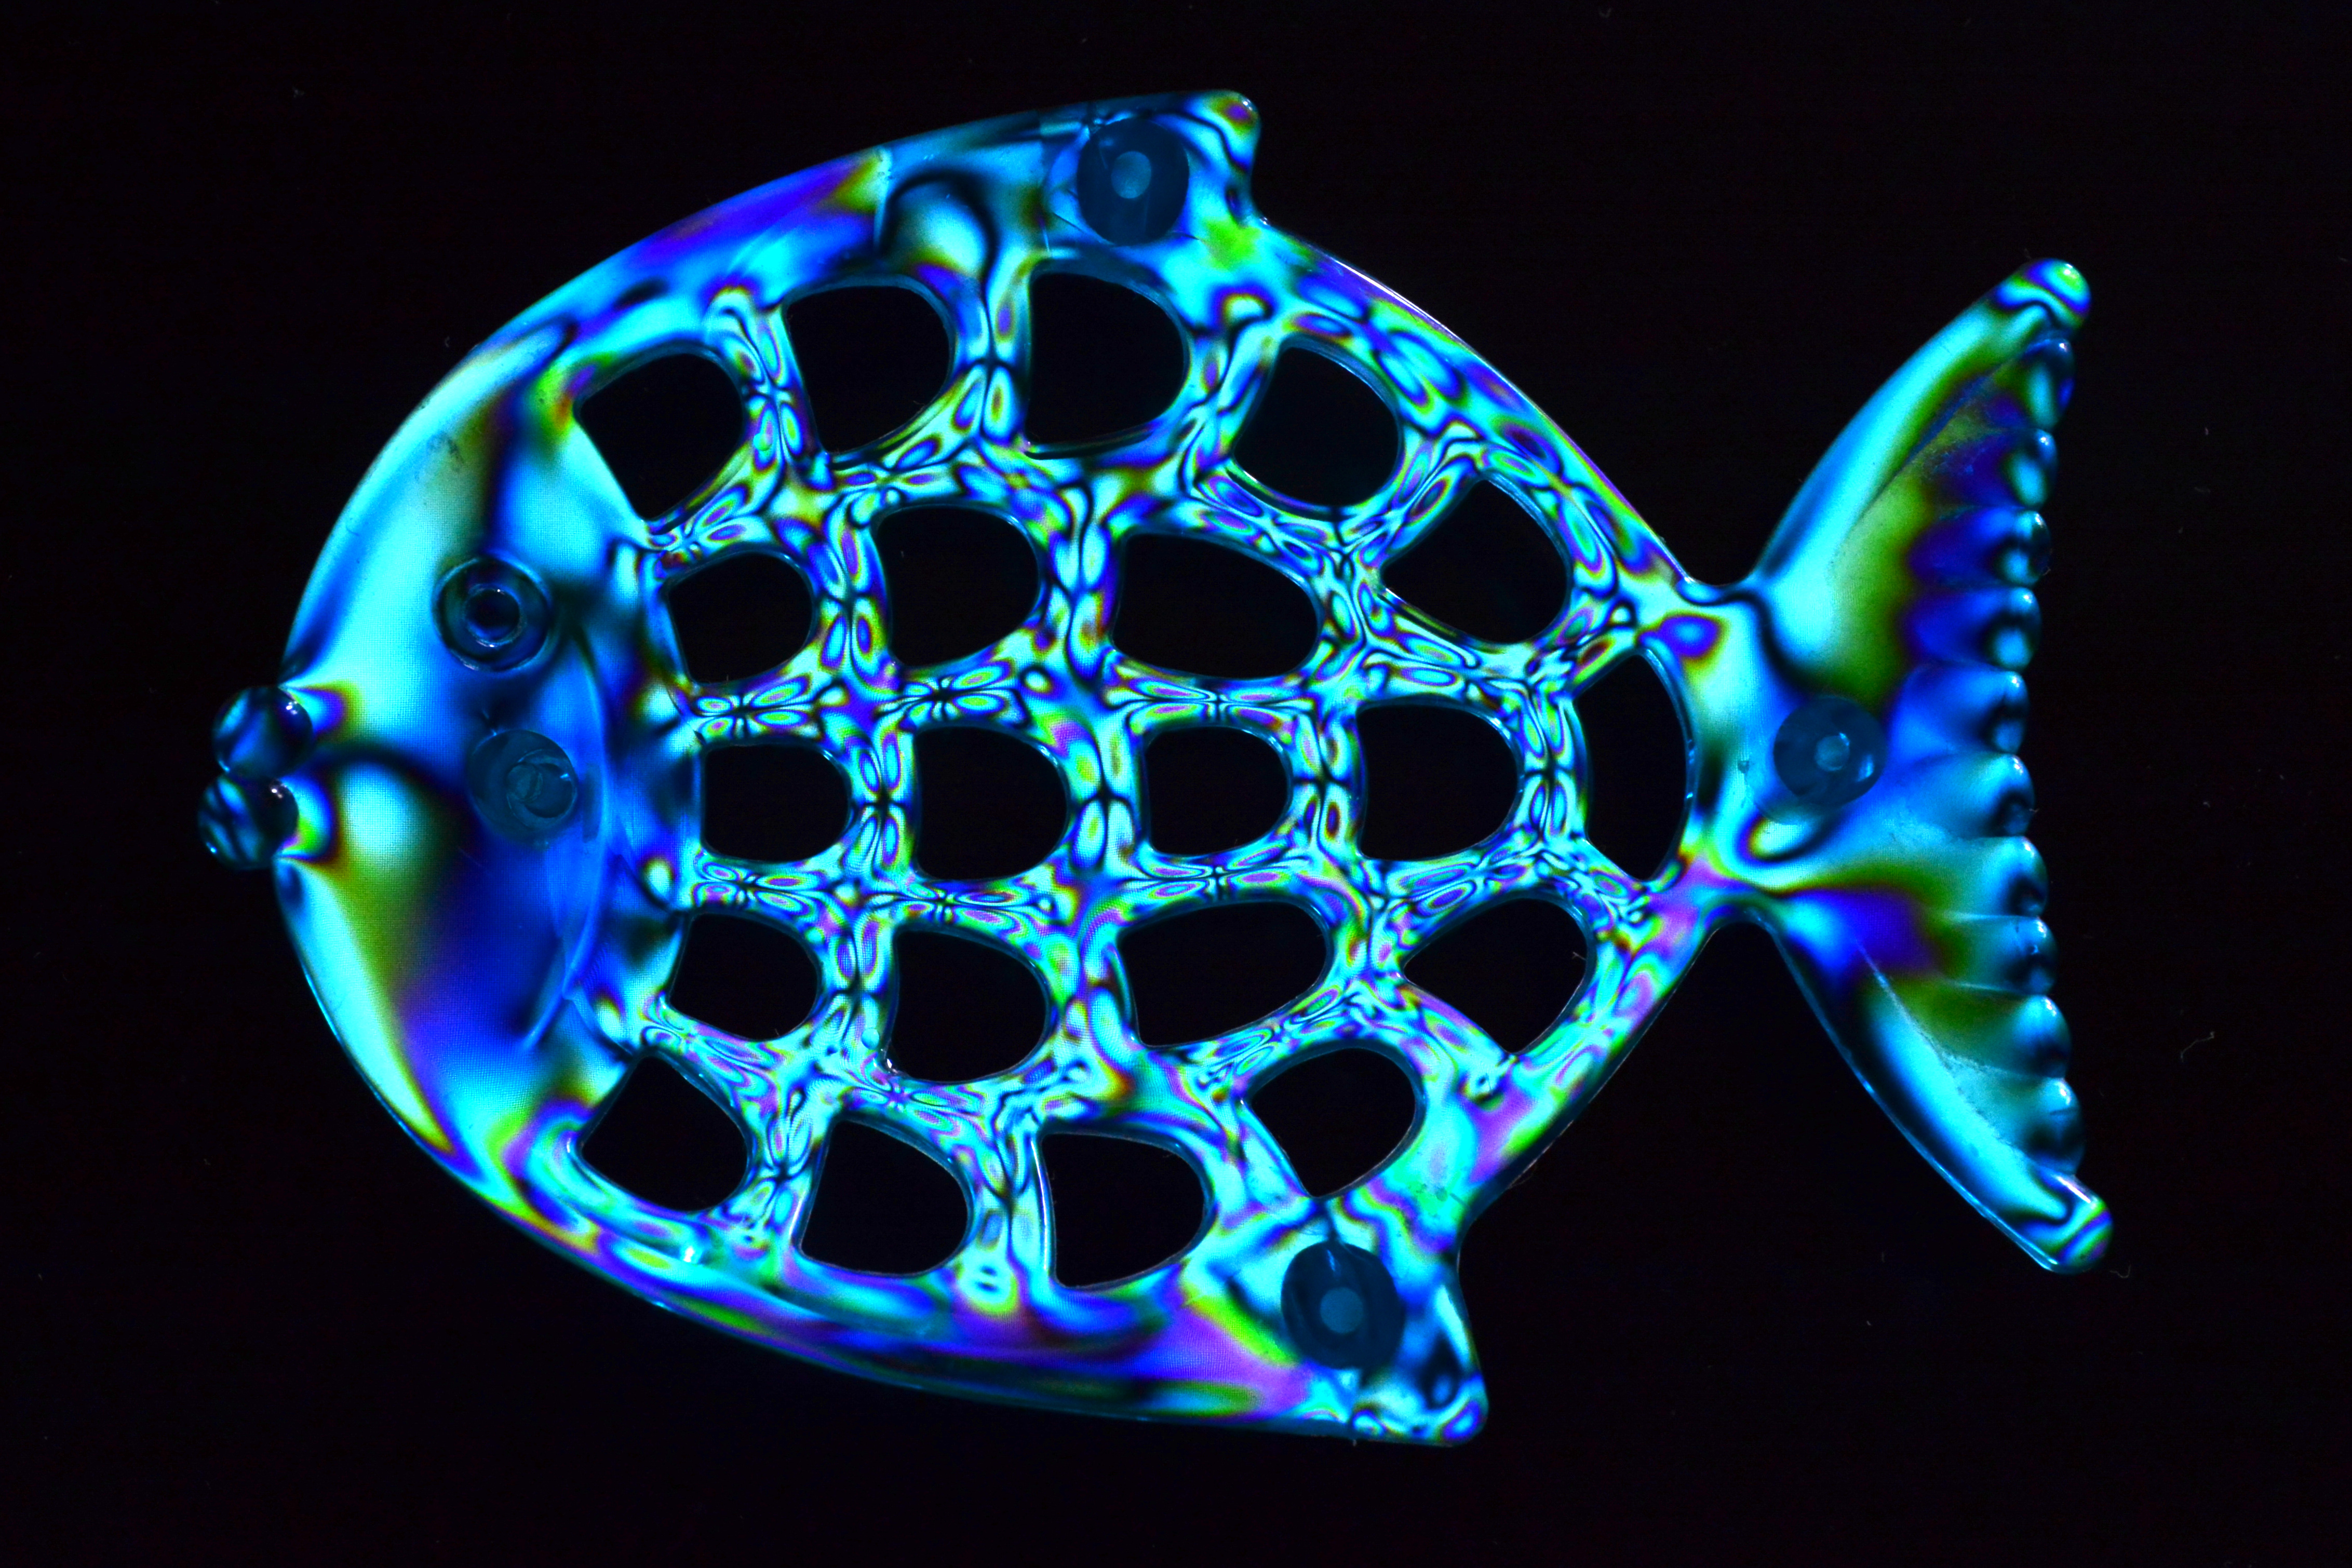
\includegraphics[width=7truecm]{slike/10_fotoelasticnost1.jpg}\hfill
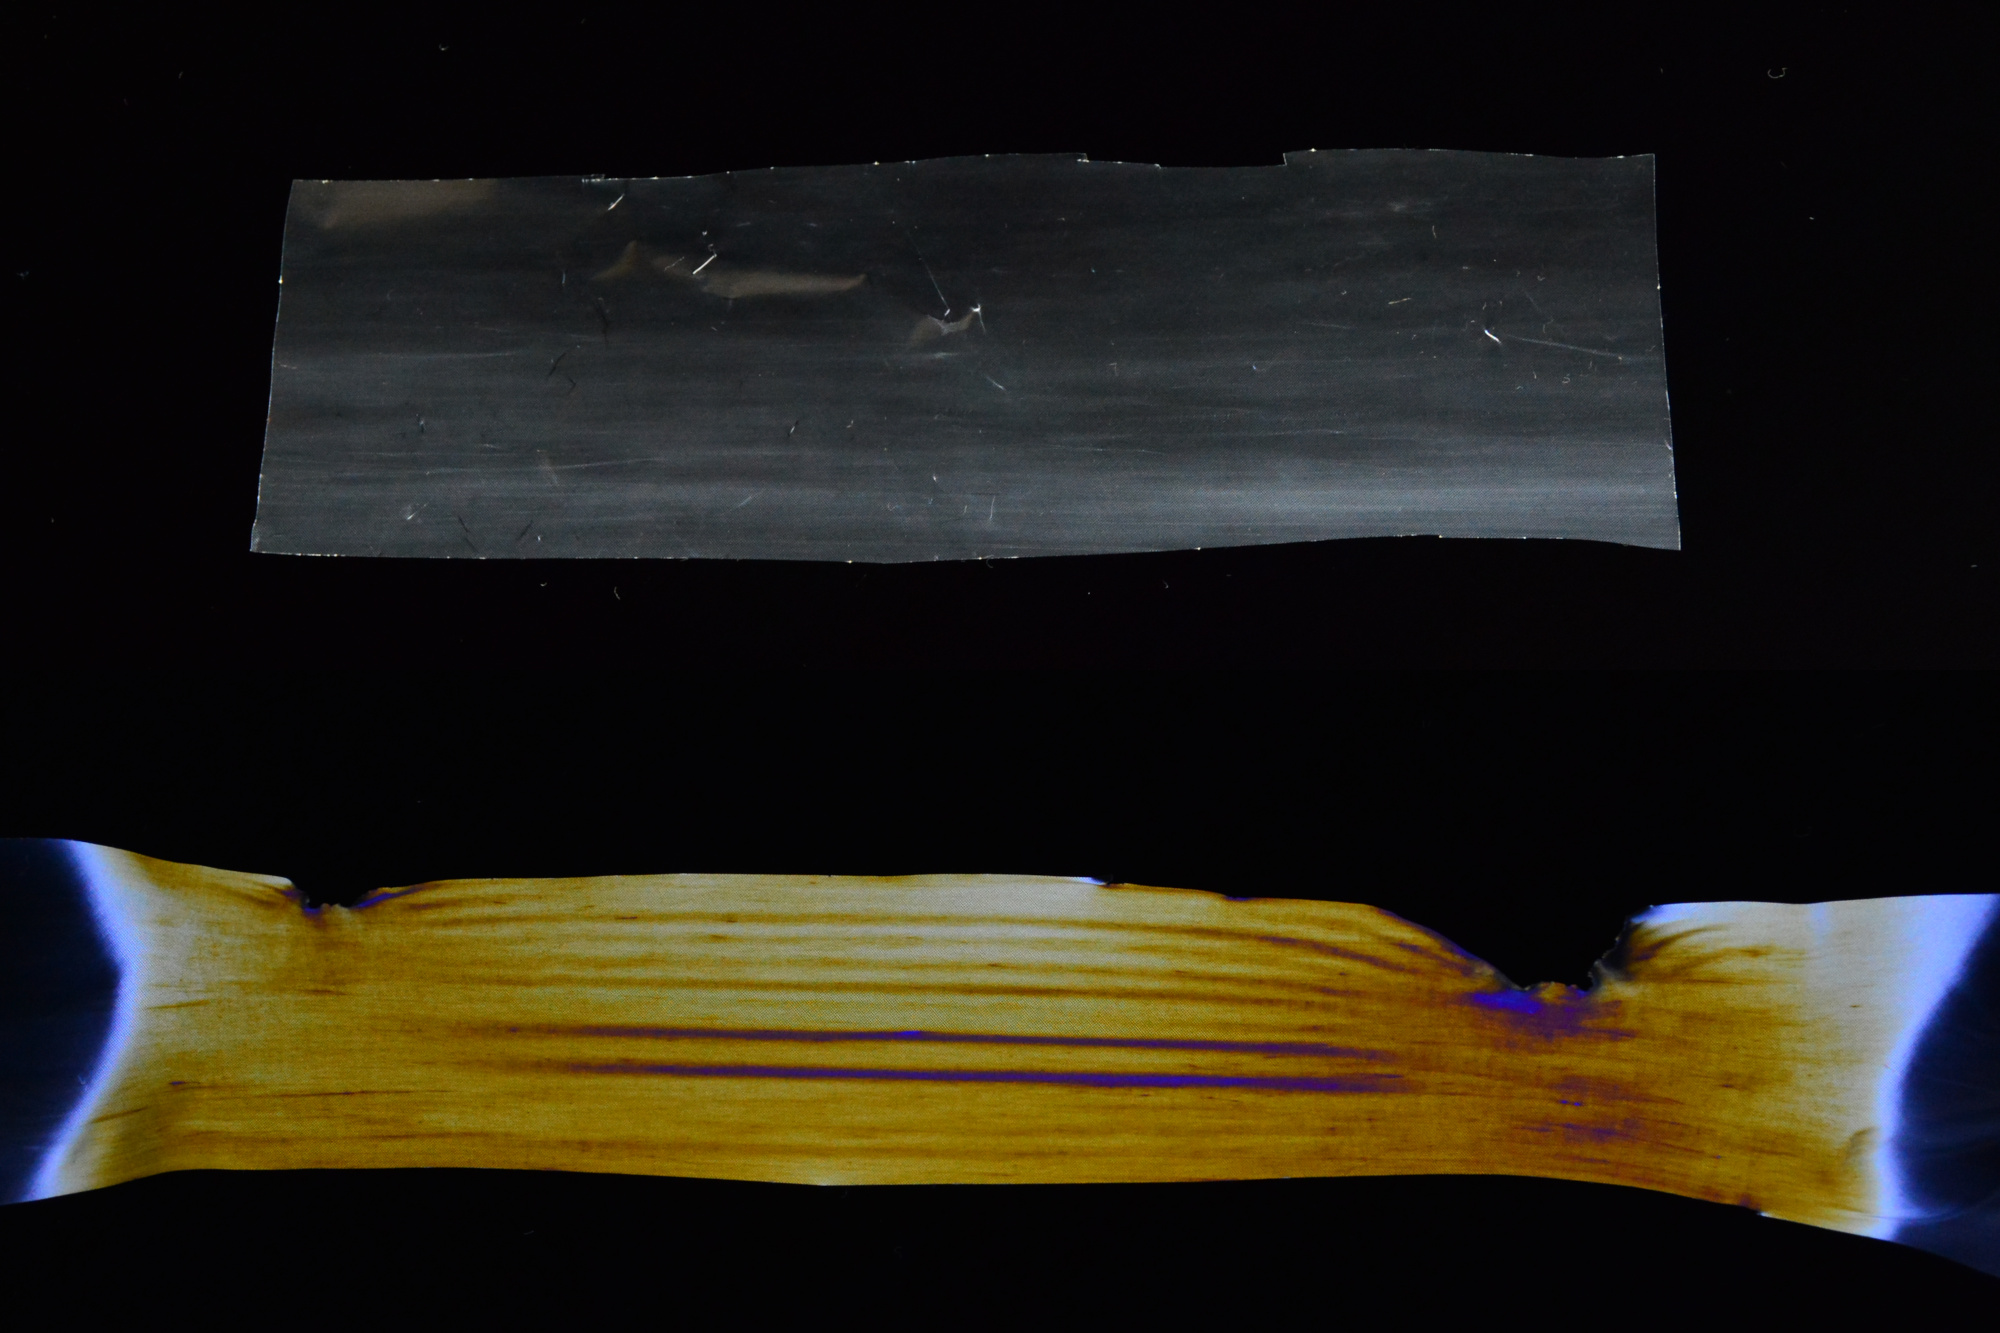
\includegraphics[width=7truecm]{slike/10_fotoelasticnost2.jpg}
\caption{Mehanske napetosti v plastičnem izdelku postanejo med prekrižanima 
polarizatorjema vidne (levo). Plastična vrečka med prekrižanima polarizatorjema (desno).
Vrečka je ki je zaradi izdelave že deloma anizotropna (zgoraj), 
pod mehansko obremenitvijo pa urejanje dolgih molekul polimera vodi 
do povečanja anizotropije (spodaj).}
\label{fig:10_fotoelasticnost}
\end{figure}

\subsection*{Elektro-optični pojav}
Na optične lastnosti snovi lahko vplivamo tudi z zunanjim električnim poljem. Omenimo 
dva pojava, to sta Pockelsov in Kerrov pojav. 

Pri Pockelsovem
pojavu je odziv snovi linearen na električno polje in je zato prisoten le v snoveh
brez centra inverzije (npr. BaTiO$_3$ ali LiNbO$_3$). Ker je inducirana anizotropija sorazmerna
s priključeno napetostjo, lahko s spreminjanjem napetosti spreminjamo fazni zamik med 
komponentama polarizacije. Z dodanim analizatorjem lahko razlike v izhodni polarizaciji
pretvorimo v razlike v intenziteti prepuščene svetlobe. Pockelsov pojav se imenuje po
nemškem fiziku Friedrichu Carlu Alwinu Pockelsu (1865--1913).

Kerrov pojav je kvadratni elektro-optični pojav in razlika v lomnih količnikih snovi 
je sorazmerna s kvadratom priključene napetosti. Snov v zunanjem polju postane
enoosna, pri čemer je optična os vzporedna zunanjemu polju. Pojav je prisoten v vseh snoveh, tudi
tekočinah, zelo izrazit je na primer v nitrotoluenu ali nitrobenzenu. Tudi v tem 
primeru s spreminjanjem priključene napetosti spreminjamo fazni zamik oziroma polarizacijo
prepuščene svetlobe. Kerrov pojav je poimenovan po škotskem fiziku Johnu Kerru (1824--1907).
